%%%% Dokumentklassen %%%%

\documentclass[a4paper,11pt,fleqn,dvipsnames,twoside,openany]{memoir} 	% Openright åbner kapitler på højresider (openany begge)

\usepackage{wrapfig}
%%%% PACKAGES %%%%
%% Oversættelse og tegnsætning %%
\usepackage[utf8]{inputenc}					% Input-indkodning af tegnsæt (UTF8)
\usepackage[danish]{babel}					% Dokumentets sprog
\usepackage[T1]{fontenc}					    % Output-indkodning af tegnsæt (T1)
\usepackage{ragged2e,anyfontsize}			% Justering af elementer
\usepackage{fixltx2e}						% Retter forskellige fejl i LaTeX-kernen
\usepackage{eso-pic}		
\newcommand\BackgroundPic{%
\put(0,0){%
\parbox[b][\paperheight]{\paperwidth}{%
\vfill
\centering
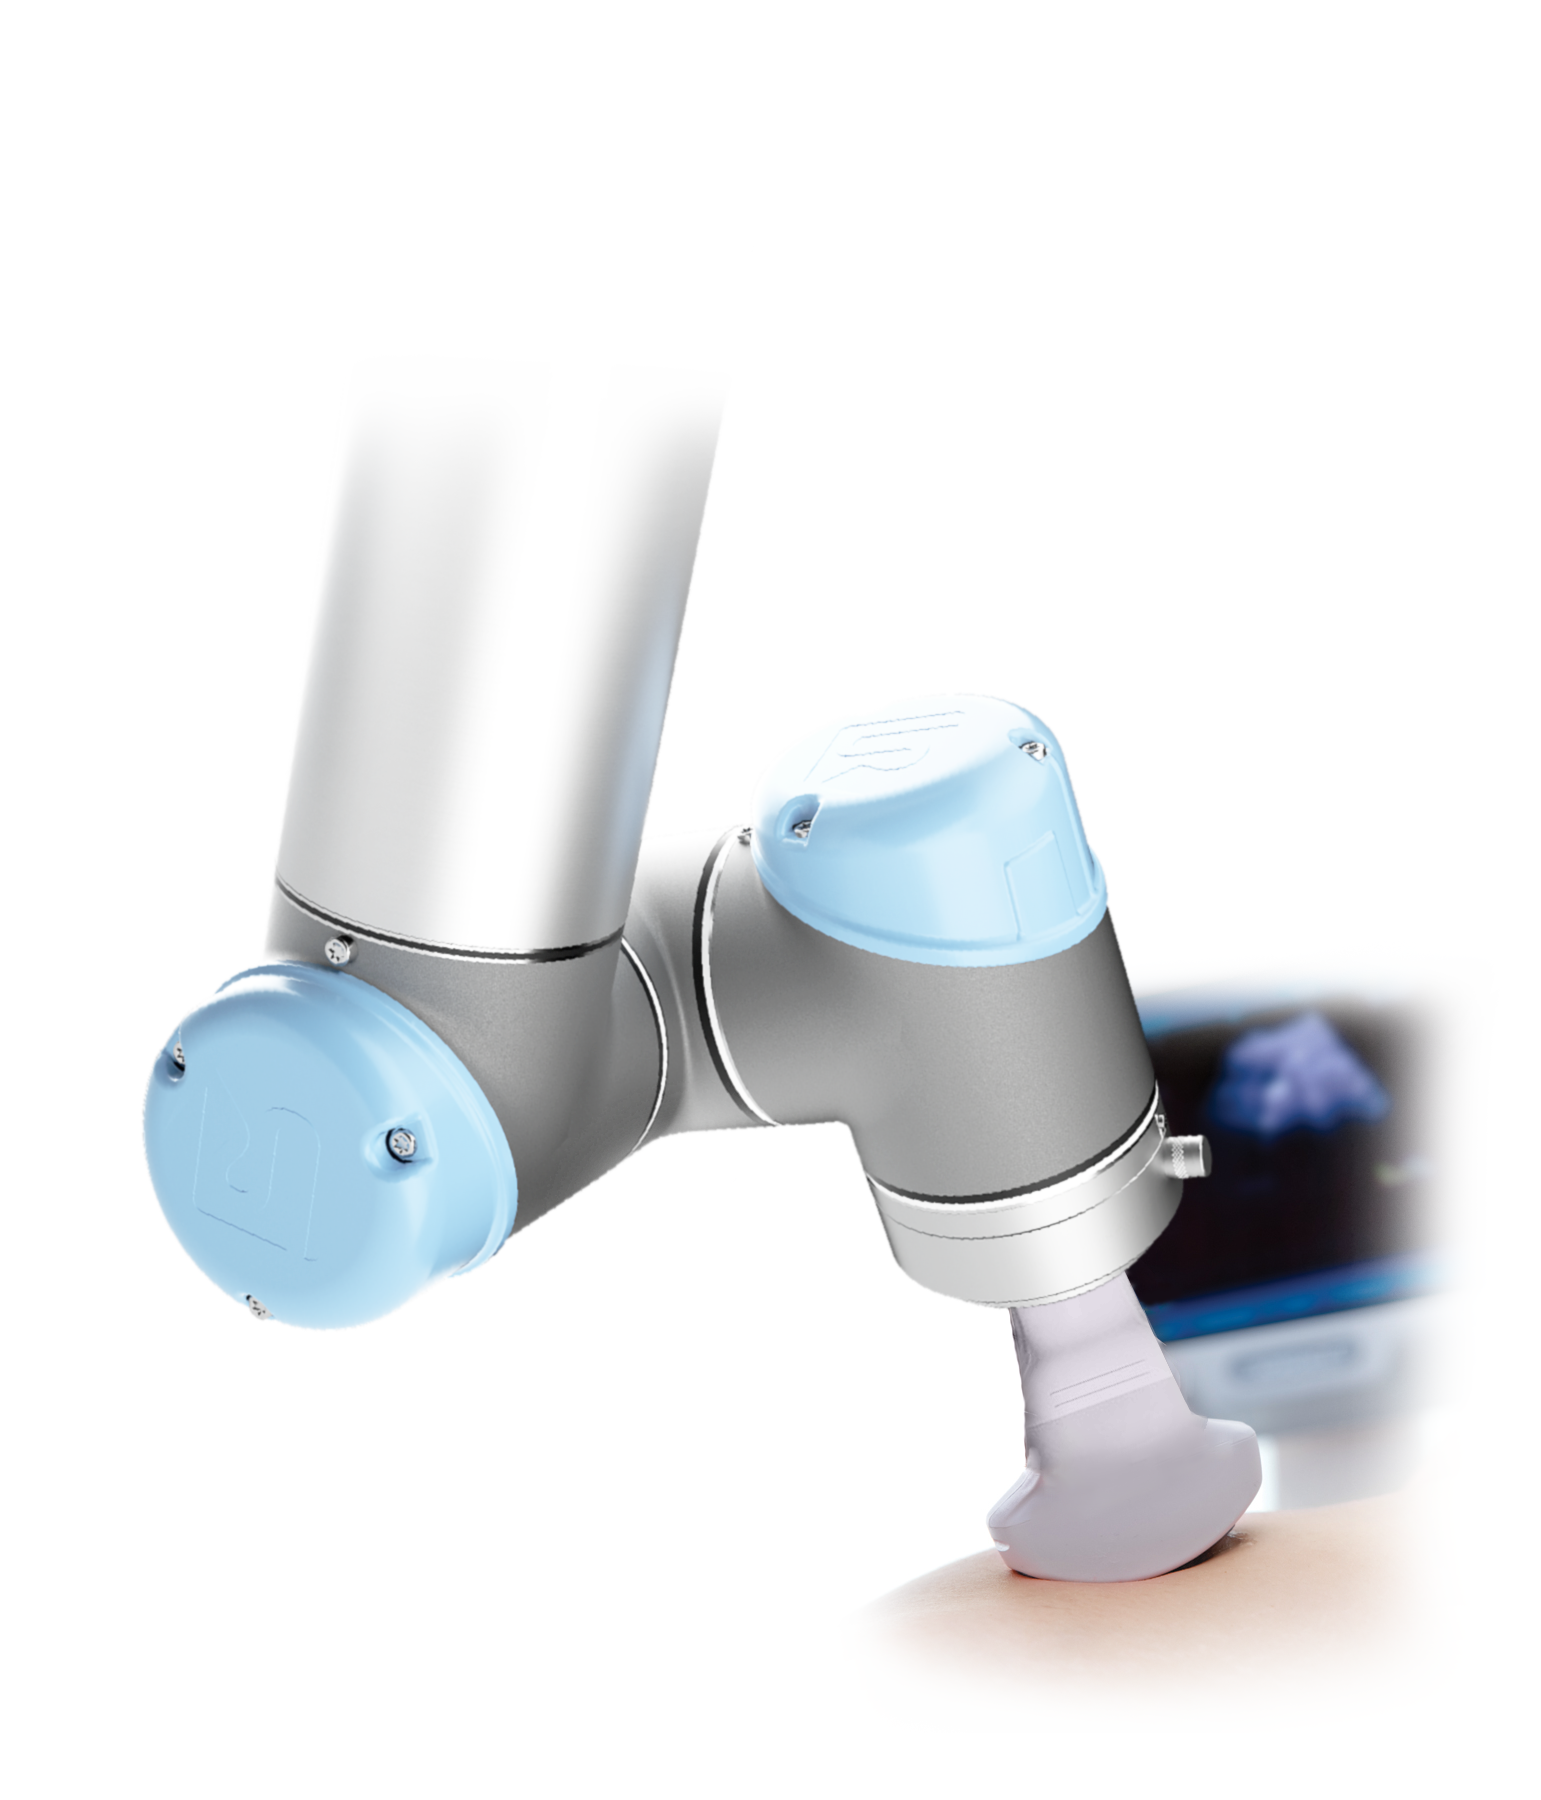
\includegraphics[width=\paperwidth,height=\paperheight,%
keepaspectratio]{figurer/forside.png}%
\vfill
}}}											
%% Figurer og tabeller (floats) %%
\usepackage{graphicx} 						% Håndtering af eksterne billeder (JPG, PNG, EPS, PDF)
\usepackage{multicol}         	            	% Muliggør output i spalter
\usepackage{rotating}						% Rotation af tekst med \begin{sideways}...\end{sideways}
\usepackage{xcolor}							% Definer farver med \definecolor. Se mere: http://en.wikibooks.org/wiki/LaTeX/Colors
\usepackage{flafter}						% Sørger for at floats ikke optræder i teksten før deres reference
\let\newfloat\relax 						% Justering mellem float-pakken og memoir
\usepackage{float}							% Muliggør eksakt placering af floats, f.eks. \begin{figure}[H]

%% Matematik mm. %%
\usepackage{amsmath,amssymb,stmaryrd} 		% Avancerede matematik-udvidelser
\usepackage{mathtools}						% Andre matematik- og tegnudvidelser
\usepackage{textcomp}                 		% Symbol-udvidelser (fx promille-tegn med \textperthousand)
\usepackage{rsphrase}						% Kemi-pakke til RS-saetninger, fx \rsphrase{R1}
\usepackage[version=3]{mhchem} 				% Kemi-pakke til flot og let notation af formler, f.eks. \ce{Fe2O3}
\usepackage{siunitx}						% Flot og konsistent præsentation af tal og enheder med \si{enhed} og \SI{tal}{enhed}
\sisetup{output-decimal-marker = {,}}		% Opsætning af \SI (DE for komma som decimalseparator) 
\usepackage{pdflscape}
\usepackage{afterpage}
%% Referencer og kilder %%
\usepackage[danish]{varioref}				% Muliggør bl.a. krydshenvisninger med sidetal (\vref)
\usepackage{natbib}							% Udvidelse med naturvidenskabelige citationsmodeller
\usepackage{xr}							    % Referencer til eksternt dokument med \externaldocument{<NAVN>}

%% Misc. %%
\usepackage{listings}						% Placer kildekode i dokumentet med \begin{lstlisting}...\end{lstlisting}
\usepackage{lipsum}							% Dummy text \lipsum[..]
\usepackage[shortlabels]{enumitem}			% Muliggør enkelt konfiguration af lister
\usepackage{pdfpages}						% Gør det muligt at inkludere pdf-dokumenter med kommandoen \includepdf[pages={x-y}]{fil.pdf}	
\pdfoptionpdfminorversion=6					% Muliggør inkludering af pdf-dokumenter, af version 1.6 og højere
\pretolerance=2500 							% Justering af afstand mellem ord (højt tal, mindre orddeling og mere luft mellem ord)	
\usepackage{hyperref}
%%%% CUSTOM SETTINGS %%%%
%% Marginer %%
\setlrmarginsandblock{3.5cm}{2.5cm}{*}		% \setlrmarginsandblock{Indbinding}{Kant}{Ratio}
\setulmarginsandblock{2.5cm}{3.0cm}{*}		% \setulmarginsandblock{Top}{Bund}{Ratio}
\checkandfixthelayout 						% Oversætter værdier til brug for andre pakker

%% Afsnitsformatering %%
\setlength{\parindent}{0mm}           		% Størrelse af indryk
\setlength{\parskip}{3mm}          			% Afstand mellem afsnit ved brug af double Enter
\linespread{1,1}							% Linjeafstand

%% Indholdsfortegnelse %%
\setsecnumdepth{subsection}		 			% Dybden af nummererede overskrifter (part/chapter/section/subsection)
\maxsecnumdepth{subsection}					% Dokumentklassens grænse for nummereringsdybde
\settocdepth{subsection} 					% Dybden af indholdsfortegnelsen
		
%% Opsætning af listings %%
\definecolor{commentGreen}{RGB}{34,139,24}
\definecolor{stringPurple}{RGB}{208,76,239}

\lstset{language=Matlab,					    % Sprog
	basicstyle=\ttfamily\scriptsize,		    % Opsætning af teksten
	keywords={for,if,while,else,elseif,		% Nøgleord at fremhæve
			  end,break,return,case,
			  switch,function},
	keywordstyle=\color{blue},				% Opsætning af nøgleord
	commentstyle=\color{commentGreen},		% Opsætning af kommentarer
	stringstyle=\color{stringPurple},		% Opsætning af strenge
	showstringspaces=false,					% Mellemrum i strenge enten vist eller blanke
	numbers=left, numberstyle=\tiny,		    % Linjenumre
	extendedchars=true, 					    % Tillader specielle karakterer
	columns=flexible,						% Kolonnejustering
	breaklines, breakatwhitespace=true,		% Bryd lange linjer
}

%% Navngivning %%
\addto\captionsdanish{
	\renewcommand\appendixname{Appendiks}
	\renewcommand\contentsname{Indholdsfortegnelse}	
	\renewcommand\appendixpagename{Appendiks}
	\renewcommand\appendixtocname{Appendiks}
	\renewcommand\cftchaptername{\chaptername~}		% Skriver "Kapitel" foran kapitlerne i indholdsfortegnelsen
	\renewcommand\cftappendixname{\appendixname~}	% Skriver "Appendiks" foran appendiks i indholdsfortegnelsen
}

%% Kapiteludssende %%
\definecolor{numbercolor}{gray}{0.7}		            % Definerer en farve til brug til kapiteludseende
\newif\ifchapternonum

\makechapterstyle{jenor}{					        % Definerer kapiteludseende frem til ...
  \renewcommand\beforechapskip{0pt}
  \renewcommand\printchaptername{}
  \renewcommand\printchapternum{}
  \renewcommand\printchapternonum{\chapternonumtrue}
  \renewcommand\chaptitlefont{\fontfamily{pbk}\fontseries{db}\fontshape{n}\fontsize{25}{35}\selectfont\raggedleft}
  \renewcommand\chapnumfont{\fontfamily{pbk}\fontseries{m}\fontshape{n}\fontsize{1in}{0in}\selectfont\color{numbercolor}}
  \renewcommand\printchaptertitle[1]{%
    \noindent
    \ifchapternonum
    \begin{tabularx}{\textwidth}{X}
    {\let\\\newline\chaptitlefont ##1\par} 
    \end{tabularx}
    \par\vskip-2.5mm\hrule
    \else
    \begin{tabularx}{\textwidth}{Xl}
    {\parbox[b]{\linewidth}{\chaptitlefont ##1}} & \raisebox{-15pt}{\chapnumfont \thechapter}
    \end{tabularx}
    \par\vskip2mm\hrule
    \fi
  }
}											        % ... her

\chapterstyle{jenor}						        % Valg af kapiteludseende - Google 'memoir chapter styles' for alternativer

%% Sidehoved %%

\makepagestyle{AAU}							        % Definerer sidehoved og sidefod udseende frem til ...
\makepsmarks{AAU}{%
	\createmark{chapter}{left}{shownumber}{}{. \ }
	\createmark{section}{right}{shownumber}{}{. \ }
	\createplainmark{toc}{both}{\contentsname}
	\createplainmark{lof}{both}{\listfigurename}
	\createplainmark{lot}{both}{\listtablename}
	\createplainmark{bib}{both}{\bibname}
	\createplainmark{index}{both}{\indexname}
	\createplainmark{glossary}{both}{\glossaryname}
}
\nouppercaseheads									% Ingen Caps ønskes

\makeevenhead{AAU}{\small BAC7 Automatisk Ultralydsscanner}{}{\leftmark}	% Definerer lige siders sidehoved (\makeevenhead{Navn}{Venstre}{Center}{Hoejre})
\makeoddhead{AAU}{\rightmark}{}{\small ASE}		            % Definerer ulige siders sidehoved (\makeoddhead{Navn}{Venstre}{Center}{Højre})
\makeevenfoot{AAU}{\small \thepage}{}{}						% Definerer lige siders sidefod (\makeevenfoot{Navn}{Venstre}{Center}{Højre})
\makeoddfoot{AAU}{}{}{\small \thepage}						% Definerer ulige siders sidefod (\makeoddfoot{Navn}{Venstre}{Center}{Højre})

\copypagestyle{AAUchap}{AAU}							% Sidehoved for kapitelsider defineres som standardsider, men med blank sidehoved
\makeoddhead{AAUchap}{}{}{}
\makeevenhead{AAUchap}{}{}{}
\makeheadrule{AAUchap}{\textwidth}{0pt}
\aliaspagestyle{chapter}{AAUchap}					% Den ny style vælges til at gælde for chapters
													% ... her
															
\pagestyle{AAU}										% Valg af sidehoved og sidefod


%%%% CUSTOM COMMANDS %%%%

%% Billede hack %%
\newcommand{\figur}[4]{
		\begin{figure}[H] \centering
			\includegraphics[width=#1\textwidth]{billeder/#2}
			\caption{#3}\label{#4}
		\end{figure} 
}

%% Specielle tegn %%
\newcommand{\decC}{^{\circ}\text{C}}
\newcommand{\dec}{^{\circ}}
\newcommand{\m}{\cdot}


%%%% ORDDELING %%%%

\hyphenation{mmHg}    %% Her kan defineres ordelingen for specifikke ord med "-". De forskellige ord adskilles med mellemrum. Fx \hyphenation{er-hvervs-liv-et Himmelstrup ka-kao}. I de fleste tilfælde kan LaTeX selv stå for det.

%%%% Tilføjelser af min preample %%%%

% Booktabs:
% The booktabs package is needed for better looking tables. 
\usepackage{booktabs}

% Caption:
% For better looking captions. See caption documentation on how to change the format of the captions.
\usepackage[hang, font={small, it}]{caption}

% Hyperref:
% This package makes all references within your document clickable. By default, these references will become boxed and colored. This is turned back to normal with the \hypersetup command below.
\usepackage{hyperref}
	\hypersetup{colorlinks=false,pdfborder=0 0 0}

% Cleveref:
% This package automatically detects the type of reference (equation, table, etc.) when the \cref{} command is used. It then adds a word in front of the reference, i.e. Fig. in front of a reference to a figure. With the \crefname{}{}{} command, these words may be changed.
\usepackage{cleveref}
	\crefname{equation}{formel}{formler}
	\crefname{figure}{figur}{figurer}	
	\crefname{table}{tabel}{tabeller}
	\crefname{section}{afsnit}{afsnit}
	\crefname{chapter}{kapitel}{kapitler}

% Mine tilføjelser:
\usepackage{nameref}                      %% Bruges til at kunne referere til kapitler og afsnits navne.
\usepackage{units}                        %% Bruges til at gøre fx 1/2 samlet med: \nicefrac{1}{2}.
\usepackage{tabu, longtable}              %% Bruges til tabeller.
\setlength{\tabulinesep}{2ex}             %% Definerer linjeafstand i tabeller.
\usepackage{enumerate}                    %% Bruges til lister.
\usepackage{tabto}                        %% Giver mulighed for TAB med fx \tabto{3em}.
\usepackage[hyphenbreaks]{breakurl}       %% Bruges til websiders url'er.
\renewcommand{\UrlFont}{                  %% Definerer url-font.
\small\ttfamily}                          %
\bibliographystyle{plain}                 %% Definere bibliografien. Ses til sidst i dokumentet i kapitlet Litteratur.
\raggedbottom

\externaldocument[D-]{Dokumentation}
\externaldocument{Bilagsliste}

\begin{document}
	
\frontmatter		
\begin{titlingpage}
\begin{center}

~ \\[3cm]


\includegraphics[width=0.6\textwidth]{figurer/ASE}~\\[1cm]

\textsc{\LARGE Aarhus University School of Engineering}\\[1.5cm]

\textsc{\Large Sundhedsteknologi og Informations- og kommunikationsteknologi}\\
\textsc{\Large Bachelorprojekt}\\[0.5cm]
\textsc{\Large Projektrapport} \\[1cm]

\noindent\makebox[\linewidth]{\rule{\textwidth}{0.4pt}}\\
[0.5cm]{\Huge Automatisk Ultralydsscanner}
\noindent\makebox[\linewidth]{\rule{\textwidth}{0.4pt}}

\end{center}
Projektnummer: 16118 \newline
Charlotte Søgaard Kristensen (201371015) \newline
Mathias Siig Nørregaard  (201270810)\newline		 
Marie Kirkegaard (201370526) \newline  

\textit{Vejleder} \newline
Associate Professor\\
Michael Alrøe\\
Aarhus School of Engineering


\vfill

\begin{center}
{\large 16. december}
\end{center}


\end{titlingpage}
\begin{vplace}[0.6]
{\large \textit{Gruppemedlemmer}}
\\
\\

\noindent \begin{tabular}{ll}
	\makebox[3.0in]{\hrulefill} & \makebox[1.5in]{\hrulefill}\\
	Marie Kirkegaard (201370526) & Dato\\[8ex]% adds space between the two sets of signatures
	\makebox[3in]{\hrulefill} & \makebox[1.5in]{\hrulefill}\\
	Charlotte Søgaard Kristensen (201371015) & Dato\\[8ex]
	\makebox[3in]{\hrulefill} & \makebox[1.5in]{\hrulefill}\\
	Mathias Siig Nørregaard (201270810) & Dato\\[8ex]
\end{tabular}
\\
\\
\\
{\large \textit{Vejleder}}
\\
\\

\noindent \begin{tabular}{ll}
	\makebox[3.0in]{\hrulefill} & \makebox[1.5in]{\hrulefill}\\
	Michael Alrøe & Dato\\[8ex]
\end{tabular}
\end{vplace}


\chapter{Resumé}
\textbf{Baggrund}
I Danmark tilbydes alle kvinder i alderen 50 til 69 år en rutinemæssig mammografiscreening. Mammografimetoden kan være uhensigtsmæssig at anvende, da det, for kvinder med meget kirtelvæv, er svært at se skelne kirtelvæv fra kræftknude, på et røntgenbillede. Derfor er man i nogle tilfælde nødt til at supplere med en ultralydsundersøgelser \cite{Ultralyd}.

I fremtiden kan man forestille sig, at automatiserede ultralydsscanninger til screening for brystkræft kunne foretages med samme procedure, som man i dag udfører mammografi. Mammografi foretages af radiografer eller røntgensygeplejersker, hvorefter røntgenbillederne sendes til en radiolog, som afgør, om der skal foretages yderligere undersøgelser.

Dette bachelorprojekt handler derfor om udvikling og undersøge af muligheden for at lave automatiserede ultralydsscanninger til screening for brystkræft, som supplement til mammografi.

\textbf{Metoder}
I udviklingsprocessen er der lavet en spørgeskemaundersøgelse, Medicinsk godkendelse og en økonomiske analyse for at undersøge hvilke tiltag der skal til for at kunne realisere Automatisk Ultralydsscanner. Til at beskrive systemet bag Automatisk Ultralydsscanner er UML og sysML anvendt. 

\textbf{Resultat}
Der er udviklet en PC Applikation, som gør det muligt for 3D Kamera at konstruere en 3D model, som Robotarm efterfølgende kan føre ultralydssproben over. 

\textbf{Konklusion}
Der blev udviklet et system, som automatisk kan udføre screeninger af brystet. Manglende kendskab til MDD har gjort at Automatisk Ultralydsscanner ikke overholder loven til medicinsk godkendelse. 
\chapter{Abstract}\label{kapitel_Abstract}
\textbf{Background} \newline
All Danish women between the ages of 50 to 69 years are offered 
mammography to screen for breast cancer. This method of screening may sometimes be unsuitable, as it is hard to distinguish between glandular tissue and tumors in an x-ray image - and some women have a lot of glandular tissue. In these cases it is necessary to perform an additional ultrasonography procedure.

Nowadays, mammography procedures are carried out by radiographers, after which the x-ray images are sent to a radiologist. The radiologist then decides if additional examinations are required. It is possible to envision automatic ultrasonographic procedures which could be accomplished with the same work flow as mammography procedures.

\textbf{Methods} \newline
Elements of Scrum were used to organize the project in the development process. A user survey, a medical approval draft and an economic analysis have been produced to investigate which approaches are needed to realize Automatic Sonography. UML and SysML have been used to describe Automatic Sonography.

\textbf{Results} \newline
The system Automatic Sonography includes a PC application which utilizes a 3D camera to instruct a robot arm to move across the surface of a chest area. Automatic Sonography cannot perform a full sonographic procedure and is not medically approved. A sonographic addition to the screening program is not necessarily cost-effective.

\textbf{Discussion}\newline
It is necessary to introduce a range of optimizations for Automatic Sonography to mimic the quality of a radiologist's scanning procedure. Additionally, the introduction of the system to the Danish healthcare service remains questionable.

\textbf{Conclusion} \newline
A system, which partially meets the requirements specified according to the delimitation, has been developed. In conclusion, it is realistic to develop an automatic sonography system to screen for breast cancer.
\chapter{Forkortelser}

\begin{table}[htb]
\centering
\begin{tabular}{ | c | p{0.80\textwidth} | }
\hline
\textbf{Forkortelser} & \textbf{Forklaring} \\\hline
ASE & Aarhus School of Engineering \\\hline
BDD & Block Definition Diagram \\\hline
FURPS+ & Funkctionality, Usability, Reliability, Performance, Supportability and Ekstra \\\hline
GUI & Graphical User Interface, Grafisk brugergrænseflade \\\hline
IBD & Internal Block Diagram \\\hline
MDD & Medical Device Directive \\\hline
MoSCoW & Must, Should, Could and Would like \\\hline
QALY & Kvalitet justeret leveår  \\\hline
RCT & randomized controlled trial \\\hline
SysML & Systems Modeling Language \\\hline
UC & Use case \\\hline
UML & Unified Modeling Language \\\hline

\end{tabular}
\caption{Forkortelser}
\end{table}

\vspace{3cm}
%\chapter{Versionshistorik}\label{Versionshistorik}

\begin{table}[htb]
\begin{tabular}{ | l | l | l | p{0.49\textwidth} | }
\hline
\textbf{Version} & \textbf{Dato} & \textbf{Ansvarlig} & \textbf{Beskrivelse} \\\hline
1.0 & 2016-11-01 & CSK & Første version af udviklingsdokuement med systembeskrivelse, bdd og ibd\\\hline
1.1 & 2016-11-03 & CSK & Sekvensdiagrammer tilføjet  \\\hline
1.2 & 2016-11-04 & CSK, MSK & Forklaringer til sekvens- og klassediagrammer \\\hline
\end{tabular}
\caption{Versionshistorik}
\end{table}                    
\cleardoublepage		

\tableofcontents* % Indsætter en indholdsfortegnelse før Indledning.

\mainmatter
  
\chapter{Forord}
Dette bachelorprojekt er udarbejdet af Marie Kirkegaard, Charlotte Søgaard Kristensen og Mathias Siig Nørregaard og er det afsluttende projekt på 7. semester for diplomingeniøruddannelsen i henholdsvis Sundhedsteknologi og informations- og kommunikationsteknologi ved Aarhus University School of Engineering (ASE). Bachelorprojektet er udarbejdet i perioden 29. august 2016 til 16. december 2016 og ideen bag bachelorprojektet er opstået hos Søren Holm Pallesen, stifter og direktør for Robotic Ultrasound. 

Formålet med projektet er at undersøge muligheden for at lave automatiske og reproducerbare ultralydscanninger til screening for brystkræft. Bachelorprojektet henvender sig primært til ingeniører indenfor sundhedsteknologi samt informations- og  kommunikationsteknologi. 

Bachelorgruppen vil gerne rette en stor tak til alle som har hjulpet med sparring gennem hele projektets forløb:

\let\labelitemi\labelitemii
\begin{itemize}
\item Associate Professor, Michael Alrøe for support og engageret vejledning gennem projektforløbet.

\item Cand.scient.med. Søren Holm Pallesen for at stå til rådighed ved diverse relevante møder, og for altid at have gode ideer til projektarbejdet.

\item Radiolog og ultralydsekspert Lars Bolvig Hansen for telefoninterview og teknisk sparring på ultralydsområdet.

\item Afdelingsradiograf Tine Bisgaard for besøg og rundvisning på Røntgen- og Skanningsafdelingen på Aarhus Universitetshospital, Tage Hansen Gade. 
\end{itemize}

\section{Læsevejledning} 
Bachelorprojektet er delt op i en projektrapport og procesrapport. Projektrapporten beskriver selve projektet, hvordan problemformuleringen er løst, samt hvilke resultater der er opnået. Procesrapporten, som findes efter projektrapporten, beskriver udviklingsprocessen af Automatisk Ultralydsscanner. Dette inkluderer projektadministrationen, arbejdsfordeling, planlægning og brug af projektstyringsværktøjer. 

Der skelnes mellem navneord med stort og småt. F.eks robotarm og Robotarm, hvor Robotarm er aktøren i systemet.
I hvert afsnit er der refereret til bilag, hvor man kan finde uddybende dokumentation. Bilag til specikke dokumenter findes nederst i hver rapport, mens den fulde oversigt over alle bilag kan findes i Bilagsliste.  
                     % Her findes de nummererede kapitler modsat \frontmatter og \backmatter.
\chapter{Indledning}
\section{Baggrund}
Danmark vil i de kommende årtier få en voksende andel af ældre borgere, der vil lægge et større pres på velfærdssamfundet i Danmark. Det vil resultere i færre borgere i den arbejdsdygtige alder, da det ud fra en befolkningsfremskrivning til 2040 forventes, at andelen af personer på 65 år og derover vil udgøre omkring en fjerdedel af den samlede danske befolkning \cite{Befolk}. En sådan ændring i demografien vil betyde flere patienter med kroniske lidelser, som derved vil medføre øgede omkostninger for og pres på sundhedsvæsenet \citep{Pres}. Det er derfor nødvendigt, at se på optimerede løsninger til behandling og diagnosticering af sygdomme. 

I Danmark tilbydes alle kvinder i alderen 50 til 69 år en rutinemæssig mammografiscreening. Mammografiscreening foregår ved en røntgenundersøgelse, hvilket er billigt og effektiv \cite{Afsloring}. Metoden er dog ikke altid den mest hensigtsmæssige at anvende, da kirtelvæv og ondartede cancersvulster kan være svære at skelne fra hinanden på et røntgenbillede. Røntgenmetoden har derfor en begrænset undersøgelseseffekt ved kvinder med meget kirtelvæv. Til disse patienter suppleres røntgenbillederne med en ultralydsundersøgelse, som fortages af en radiolog \cite{Ultralyd}.

Ultralyds- og røntgenundersøgelser har hver sine fordele og kan derfor sjældent stå alene. Ultralyd har den største diagnosesikkerhed i kirtelvæv, hvor røntgen har den største diagnosesikkerhed i fedtvæv. Da brystet ofte er en kombination af de to vævstyper, supplerer disse to metoder hinanden godt \cite{Ultralyd}. 

Mammografi foretages i dag af enten en radiograf eller en røntgensygeplejerske, hvorefter røntgenbillederne bliver sendt videre til en radiolog. I fremtiden kunne det forestilles, at automatiserede ultralydsscanninger til screening for brystkræft kunne foretages med samme procedure, hvor ultralydsvideoclips efterfølgende sendes til lægen.

Dette bachelorprojekt går derfor ud på at lave et Proof of Concept, for af undersøge muligheden for automatiserede ultralydsscanninger til screening for brystkræft.
\newpage

\section{Problemformulering}
Med udgangspunkt i projektets baggrund og projektbeskrivelse, er der defineret følgende problemstillinger, som forsøges besvaret og belyst i dette bachelorprojekt. Se bilag \ref{Projektbeskrivelse} Projektbeskrivelse (ASE)

\textbf{Hvordan kan en automatiseret ultralydsscanner til screening for brystkræft udvikles samt hvilke økonomiske og produktsikkerhedsmæssige tiltag vil kunne realisere dette?}

\let\labelitemi\labelitemii
\begin{itemize}
\item Hvordan vil en automatiseret ultralydsscanning til screening for brystkræft kunne udvikles ved brug af robotarm og 3D kamera?
\item Hvilke omkostninger vil indførslen af en Automatisk Ultralydsscanner kunne give? 
\item Hvilke konsekvenser vil en tilføjelse af Automatisk Ultralydsscanner til screeningsprogrammet have?
\item Hvad kræves for at få Automatisk Ultralydsscanner CE-mærket? 
\end{itemize}

\chapter{Teori}\label{Teori}

\section{Brystets opbygning og brystkræft}
Bryster er sammensat af mange små brystkirtler, bestående af kirtelceller til producering af mælk, og udførselsgange, som samler sig frem til brystvorten. Mænds bryst er opbygget ligesom kvindebrystet, dog uden fungerende mælkekirtler \cite{Mand}. Brystkirtlerne er omgivet af fedt og bindevæv\citep{Bryst}.

\begin{figure}[H]
    \centering
    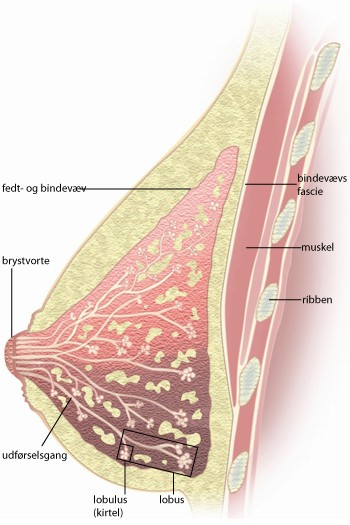
\includegraphics[width=0.35\textwidth]{figurer/r/bryst}
    \caption{Brystets opbygning \citep{Bryst}}
    \label{Brystet}
\end{figure}

I brystet kan der opstå brystkræft, hvor det hyppigst opstår i en udførselsgang \citep{Bryst}. Brystkræft er den mest udbredte kræftform hos kvinder, men den kan også opstå ved mænd,. Det er dog meget hyppigere hos kvinder \cite{Mand}.

Forstadiet til brystkræften sker ved en mutation af cellernes gener. Denne mutation kan ske over tid, men kan også være et arvet gen. Mutationen gør, at cellerne ændrer form og udseende, da cellerne deler sig for meget, hvilket danner en knude. Normalt vil syge celler nedbrydes, men dette sker ikke ved kræftceller, som hele tiden deler sig og skaber nye kræftceller. Bliver udviklingen af kræftcellerne ikke behandlet, vil kræftcellerne med tiden brede sig til det omkringliggende væv \cite{Udvikling}. 

\section{Ultralydsscanning}
Ultralyd er højfrekvent lyd, hvor man til ultralydsscanning benytter frekvenser mellem 2 og 20 kHz \cite{Frekvens}. Der anvendes en ultralydsprobe, som er en transducer. Transduceren indeholder piezoelektriske krystaller, som skaber lydbølger, når de bliver udsat for en elektrisk spænding. Disse lydbølger udsendes mange gange i sekundet fra transduceren og reflekteres tilbage til transduceren, når de møder væv. Ud fra lydbølgerne, transduceren modtager, dannes en ultralydsscanning, som lægen kan diagnosticere ud fra \cite{Ultralydsscanning}.

På scanningen ses kirtelvæv som lyst, og kræftknuder fremtræder som mørke områder.  Der er derfor en god kontrast mellem kirtelvæv og kræftknude på et ultralydsbillede \citep{Ultralyd}.

\section{Røntgenundersøgelse}
Røntgenstråler er elektromagnetiske bølger med en kortere bølgelængde end synligt lys. Strålerne er ioniserede, og derfor er det vigtigt at give den korrekte dosis, der måles med enheden milliSievert (mSv). Ved mammografiscanninger med røntgen benyttes en dosis på 0,5 mSv. \cite{Sundhedsstyrelsen}. Livstidsrisikoen for at inducere kræft efter en mammografiscanning med røntgen er definieret som meget lille, hvilket betyder, at 1 ud af 100.000 til 1 ud af 10.000 rammes \cite{Risk}. 

Ved røntgenundersøgelser sendes røntgenstrålerne fra et røntgenrør gennem patienten og opfanges på en fotografisk film, som vil danne billedet alt afhængig af, hvor meget af strålingen, der bliver absorberet i kroppen. \cite{Rontgenundersogelse}

På røntgenbilleder ses fedt og andre bløddele som grå skygger, da de ikke absorberer så mange røntgenstråler. Hvorimod kræftknuder absorberer meget røntgenstråling og derfor ses som lyse områder. \cite{Rontgenundersogelse}

På figur \ref{rontgen} ses et røntgenbillede af brystvæv. Kræftknuden ses tydeligt som den lysende plet, markeret med en firkant. Billedet i figur \ref{ultralyd} viser et stilbillede af en ultralydsscanning af brystvæv. På billedet ses kræftknuden som en mørk skygge. 

\begin{figure}[H]
    \centering
    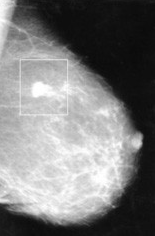
\includegraphics[width=0.40\textwidth]{figurer/r/rontgen}
    \caption{Røntgenbillede af brystvæv, hvor knuden ses inde i firkanten \cite{Mammografi}}
    \label{rontgen}
\end{figure}


\begin{figure}[H]
    \centering
    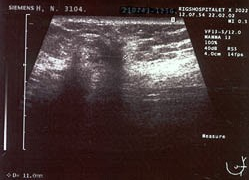
\includegraphics[width=0.40\textwidth]{figurer/r/ultra}
    \caption{Ultralydsbillede af brystvæv, hvor knuden ses som de mørke skygger \cite{Ultralyd}}
    \label{ultralyd}
\end{figure}
\chapter{Afgrænsning}
\label{Afgransning}

I udviklingsforløbet blev det besluttet ikke at inkludere eksterne sensorer eller software til målingen af påført tryk, og dermed har det ikke være nødvendigt at have en ultralydsscanner til rådighed. Det er i stedet valgt at prioritere 3D kameraets genkendelse af dybde i brystområdet, og derefter bruge billedet til at få robotarmen til at bevæge sig rundt på det detekterede område. Det blev bedømt at disse elementer var vigtigere at implementere, for at udføre et Proof of Concept.

Der er i projektet blevet benyttet et 3D kamera af typen Microsoft Kinect for Windows v2 sensor, som er et forholdsvis et stort kamera. Det blev vurderet at det ville være besværligt at have både en ultralydsprobe og en Kinect monteret på robotarmen på samme tid. Det er derfor valgt at montere 3D kameraet i loftet. 

Armhulerne scannes også ved en konventionel ultralydsscanning af brystet. Det er valgt at afgrænse til scanning af brystet, da armhulerne besværgerliggører operatørs beskærimg af 3D scanningen. Scanning af armhuler vil resultere i en 3D model af uinteressante områder, hvorfor brystområdet er valgt som afgrænsning.  

\chapter{Systemkrav}\label{Systemkrav}
\section{Systembeskrivelse}
Automatisk Ultralydsscanner er et system, som gør det muligt at lave en automatiseret ultralydscanning af brystet mhp. screening for brystkræft. Systemet Automatisk Ultralydsscanner består af Robotarm, PC Applikation med en grafisk brugergrænseflade (GUI), 3D kamera og Ultralydsscanner. Se figur \ref{Systembeskrivelse} nedenfor. 

Via GUI kan en operatør, med kendskab til ultralyd, interagere med en PC applikation. Operatøren vælger først at udføre en 3D-scanning af patientets bryst. Derefter kan PC applikationen, ud fra 3D scanningen, udregne de positioner og rotationer der er nødvendige for at udføre en ultralydsscanning. For at kunne ultralydsscanne er det nødvendigt at påføre ultralydsgel. Dernæst vil operatøren vælge at påbegynde ultralydsscanningen, hvor en robotarm med påmonteret ultralydsprobe føres rundt på det detekterede brystområde på patienten. Ultralydsscanningsvideoen kan herefter sendes til undersøgelse.

Figur \ref{Systembeskrivelse} nedenfor viser en oversigt over, hvordan elementerne i Automatisk Ultralydsscanner interagerer med hinanden.
 
\begin{figure}[H]
    \centering
    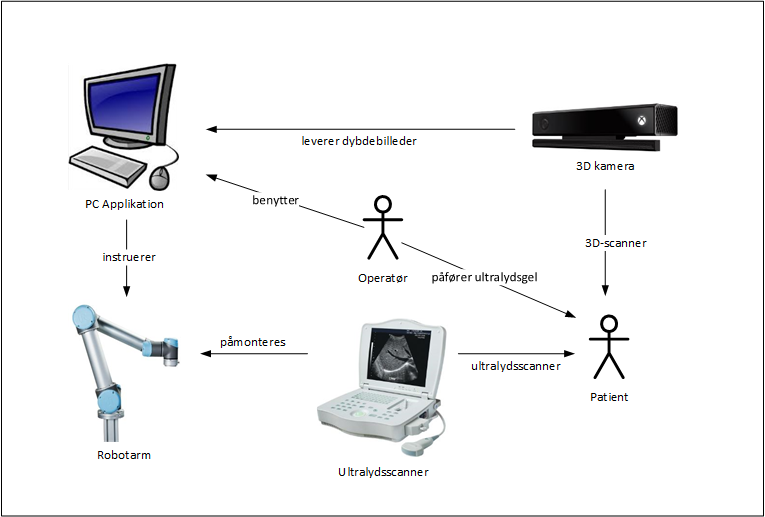
\includegraphics[width=0.75\textwidth]{figurer/d/Kravspecifikation/Systembeskrivelse}
    \caption{Systemoversigt over Automatisk Ultralydsscanner, der beskriver systemets opbygning og hvorledes de enkelte elementer interagerer}
    \label{Systembeskrivelse}
\end{figure}

\section{Aktører}
Der er identificeret fem aktører, som interagerer med systemet. Aktørerne inkluderer en operatør, en patient, en robotarm, en ultralydsscanner og et 3D kamera. PC Applikation ses som værende én samlet blok af PC og software, hvor softwaren er på PC. Operatør betjener PC Applikation, mens scanningen foregår på Patient. 3D kamera leverer dybdebilleder til PC Applikation. Robotarm styrer en påmonteret Ultralydsscanner i et specifikt overlappende bevægelsesmønster på det detekterede område.

\section{Funktionelle krav}
De funktionelle krav for Automatisk Ultralydsscanner er defineret ved brug af use cases (UC). Til systemet er der identificeret fire use cases, som kan ses i use case diagrammet på figur \ref{UseCaseDiagram} og i kravspecifikation, bilag \ref{Kravspecifikation}. 

Operatør gør klar til scanning ved at opstarte system (UC1: Start System). Hovedmenuen på GUI vil vises, hvorpå Operatør kan vælge at 3D scanne Patients brystområde (UC2: 3D scan brystområde). Inden der kan ultralydsscannes, skal Operatør påføre en gel for at muliggøre ultralydsscanning. Operatøren har mulighed for at vælge at lave en ultralydsscanning ved tryk på en knap på GUI, hvorefter Robotarm vil køre over brystet (UC3: Ultrascan brystområde).  Operatør kan derefter på GUI vælge at stoppe systemet (UC4: Stop System). 

\begin{figure}[H]
    \centering
    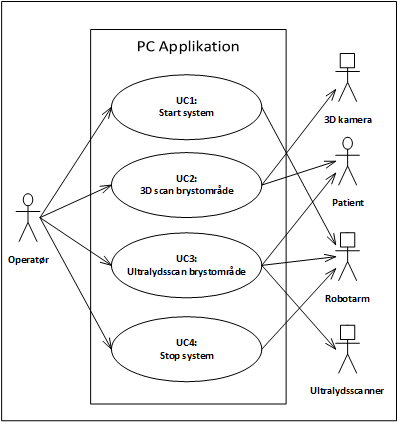
\includegraphics[width=0.75\textwidth]{figurer/d/Kravspecifikation/UseCaseDiagram}
    \caption{Use case diagram for Automatisk Ultralydsscanner, der viser systemets funktionaliteter og aktørernes relation hertil.}
    \label{UseCaseDiagram}
\end{figure}

\section{Ikke-funktionelle krav}
De ikke-funktionelle krav for Automatisk Ultralydsscanner er beskrevet ved brug af MoSCoW og FURPS+. Det er kun must-krav der er implementeret og specielt performancestider for Automatisk Ultralydsscanners er prioriteret, for at systemet kan udføre en scanning på samme tid som en radiolog. Nedenfor kan de implementerede ikke-funktionelle krav ses. 

\subsubsection{Usability}
\begin{itemize}
    \item [U1.] PC Applikation skal have en GUI. (must)
     \item[U2.] GUI skal have en procent-indikator for ultralydsscanningens gennemløb. (must)
\end{itemize}

\subsubsection{Performance}
\begin{itemize}
    \item[P1.] Scaningen med 3D kamera og ultralydsscanning skal max tage 10 minutter til sammen. (must) 
    \item[P2.] Starttid på PC Applikation skal være max 10 sekunder. (must)
    \item[P3.] 3D kamera skal max bruge 10 sekunder på at tage 3D billedet. (must)
    \item[P4.] PC Applikation skal max 10 sekunder på at færdiggøre brystområdets positurer til Robotarm. (must)
\end{itemize}

\subsection{Ekstra}
Lovkravene til medicinsk udstyr og software til medicinske udstyr, burde have været et must-krav i de ikke-funktionelle krav til Automatisk Ultralydsscanner, men da den medicinske godkendelse først blev udarbejdet sent i udviklingsprocessen er kravene fra den medicinske godkendelse ikke implementeret i systemet. Dette er for eksempel krav som at Automatisk Ultralydsscanner skal: 

\begin{itemize}
\item Designes så det ikke er til fare for Operatør og Patient. 
\item Fremstilles i et materiale som mindsker spredning af bakterier. 
\item Have tydelige og letforståelige tegn på knapper og display.
\item Have et risikohåndteringssystem.
\item Have kvalitetssikringssystem. 
\item Mærkes så der ikke kan være tvivl om hvordan produktet skal bruges.
\item Kunne modstå en luftbåren ESD-transient på op til ±8 kiloVolt
\item Kunne tåle en indstråling på 3V/m
\end{itemize}
\chapter{Metoder}\label{Metoder}

Til udviklingen af dokumentation for Automatisk Ultralydsscanners design, er der brugt arbejdsværktøjerne Unified Modeling Language (UML) \cite{UML}  og Systems Modeling Language (SysML) \cite{SysML}. Projektarbejdet har bestået af udvikling af software, hvor UML er benyttet til at opstille bl.a. use cases, aktør-kontekst diagrammer samt sekvens- og klassediagrammer mm. Systemet anvender allerede udviklet hardware, som PC applikationen skal have forbindelse til. SysML er benyttet til at lave block definition diagram (BDD) og internal block diagram (IBD) til at illustrere forbindelsen mellem de forskellige komponenter som f.eks. robotarmern.

Der er anvendt kvalitative og kvantitative metoder \cite {MetoderBruger} til brugerundersøgelser, hvor den kvalitative primært er brugt til at øge forståelsen i interviews, mens den kvantitative er brugt til at lave statistik på spørgeskema. En break-even analyse \cite{Erhvervsokonomi} er benyttet som værktøj til at give en forståelse for, hvordam omkostninger reagerer ift. ændringer af transportvariabler. Litteratursøgning med søgeprotokol er benyttet til at finde litteratur om screeningsprogrammer. Se afsnit \ref{Analyser} Analyser, for anvendelsen af metoderne. 

Til udarbejdelsen af medicinsk godkendelse af Automatisk Ultralydsscanner er der benyttet direktiver og tilhørende standarder til at beskrive, hvordan man CE-mærker, og hvordan godkendelsesproceduren kan gennemføres.  Se afsnit \ref{MedicinskGodkendelse} Medicinsk godkendelse, for analysen. 

Til udarbejdelse af produktet og tilhørende krav, design og test, er der blevet anvendt elementer af Scrum, V-modellen og en tidsplan. For at læse mere om brugen af disse værktøjer, se procesrapporten, der følger denne rapport.


\chapter{Analyser}\label{Analyser}

\section{Brugerundersøgelse}
Der er foretaget to slags brugerundersøgelse, en kvantitativ med potentielle patienter og to kvalitative interviews med en overlæge og en specialeansvarlig radiograf. Dette er medtaget for at belyse, hvordan vil en automatiseret ultralydsscanner til screening for brystkræft modtages af patienter og personale. 

\subsection{Spørgeskemaundersøgelse}
Undersøgelsen bestod af et kvalitativt spørgeskema med tre spørgsmål, omhandlende scanning med en automatiseret robotarm fremfor en læge, samt hvilke problemstillinger og fordele respondenterne ser ved en automatiseret ultralydsscanner. Spørgeskemaundersøgelsen blev lavet før projektet var færdigdefineret og derfor falder den lidt ved siden af projektet, den er dog stadig medtaget i projektet, fordi den kan give et billede af, hvordan patienter vil tage imod Automatisk Ultralydsscanner.  

Der var i alt 72 respondenter på spørgeskemaet, hvor størstedelen, 87,5\%, af respondenterne var positive for at blive scannet af robotarmen hvis kvaliteten og sikkerhed er på højde med, hvad den er, når en læge foretager en ultralydsscanningen. De sidste 12,5\% som var negative for automatisk scanning med en robotarmen frygter, at robotarmen vil lave fejl, det bliver upersonligt, og at det vil give en fornemmelse af, at lægen har berøringsangst for patienterne. 
De problemstillinger respondenterne ser ved automatiserede ultralydsscanninger, var at robottens følsomhed mangler, og det måske kan gøre undersøgelsen ubehagelig og utryg for patienten. Samtidig nævner flere bekymringer for robottens evne til at scanne forskellige kropstyper. Fordelene, som respondenterne så ved automatiserede ultralydsscanninger var, at robotten måske kan give økonomisk mening med kortere ventetider og spare tid og dermed frigøre ressourcer i form af personale til andre opgaver. Flere af respondenter mente, at en robotarm kan reproducere scanningerne og er derfor ikke afhængig af, hvor god lægen er. Den yngre del af respondenterne nævner ergonomiske fordele for lægen, mindre blufærdighed og langdistance-undersøgelser, som andre fordele. 

Se bilag \ref{Sporgeskemaundersogelse} Spørgeskemaundersøgelse, for hele spørgeskemaundersøgelsen. 

\subsection{Besøg og interview på Aarhus Universitetshospital, Tage-Hansens Gade} 
Aarhus Universitetshospital, Tage-Hansens Gade blev kontaktet til inspiration og belysning af den daglige praksis på en røntgen- og skanningsafdeling, samt undersøgelse af sundhedsfagliges meninger om Automatisk Ultralydsscanner. Radiograf Tine Bisgaard indvilgede i at vise rundt på afdelingen samt svare på spørgsmål om afdelingens dagligdagen. På daværende tidspunkt var Automatisk Ultralydsscanner ikke afgrænset til at kunne indgå i som supplement til mammografi i screeningspakken. 

Tine Bisgaard vurderede mammografi af begge bryster til at tage 5 minutter, mens en ultralydsscanning blev vurderet til at tage omkring 10 minutter, afhængigt af radiologens rutine. Tine Bisgaard mente ikke, at det vil være et problem at benytte en Automatisk Ultralydsscanner til at udføre scanninger, hvis man blot informerer patienterne. Hun ser dog en ulempe ved at lade en radiograf lave scanningerne idet, patienten ikke kan få svar med det samme, hvilket de normalt får når en radiolog udføre ultralydsscanningen. Tine Bisgaard nævnte yderligere en ulempe, hun frygter at det vil tage længere tid at foretage scanningen og derefter få en radiolog til at vurdere billederne.

Fordelene, Tine Bisgaard ser ved en Automatisk Ultralydsscanner er, at man på afdelingerne er nødt til at tænke i nye baner i forhold til manglen på radiologer i Danmark. Derfor mener hun, at det vil være smart, hvis radiograferne kunne udføre en del af arbejdet med ultralyd for at spare tid og penge. Tine Bisgaard og en unavngiven kollega på afdelingen foreslår, at proceduren kan gøres simpel, dvs. gøre svare kvantitative f.eks. mål, ja/nej. Det ser hun som måden en radiograf vil kunne styre en Automatisk Ultralydsscanner. På baggrund af interviewet og rundvisningen på afdelingen, blev der i projektet fokus på, hvordan en procedure for Automatisk Ultralydsscanner kukke gøre simpel, og om substitueringen af radiologer med radiografer ville kunne være en økonomisk gevinst. Derudover blev det besluttet at Automatisk Ultralydsscanner max måtte være 10 minutter om at udføre 3D scanning og efterfølgende ultralydsscanning. 

Se bilag \ref{Tine} Interview med afdelingsradiograf Tine Bisgaard, for hele interviewet. 

\subsection{Interview med radiolog og ultralydsekspert}
Der blev foretaget et telefonisk interview og efterfølgende et opfølgende møde med radiolog og ultralydsekspert, Lars Bolvig. Interviewet blev lavet for at undersøge proceduren ved ultralydsscanninger af brystet. Der var på forhånd defineret nogle spørgsmål angående lokalisering af knuder, hastigheder og tiden en læge typisk vil bruge på en ultralydsscanning af brystet og lokalisering af knuder. Ifølge Lars Bolvig vil en læge kunne lokalisere en knude i brystet på 2-3 minutter, mens hastigheden, der scannes med, er meget operatørafhængig. Lars Bolvigs forslag til hvor det vil give mening at implementere Automatisk Ultralydsscanner var til supplement til mammografi. Det vil sige, at Automatisk Ultralydsscanner vil kunne give mening at implementere som en udbyggelse af screeningsproceduren med mammografi, som anvendes i dag. Dette kunne give mening fordi, at man med en efterfølgende ultralydsscanning, efter en mammografiundersøgelse, vil kunne opdage flere kræfttilfælde. 

Lars Bolvig fortalte, at ved ultralydsscanning af brystet, føres ultralydsproben i en sinus-lignende kurve hen over brystet. Probens bane skal overlap og man tager et bryst af gangen. Det skal sikres, at ultralydsproben starter og slutter uden for brystvævet, for at sikre at at hele brystet er scannet. Bevægelsesmønsteret er illustreret i Figur \ref{Probensbevagelse} nedenfor. 

\begin{figure}[H]
    \centering
    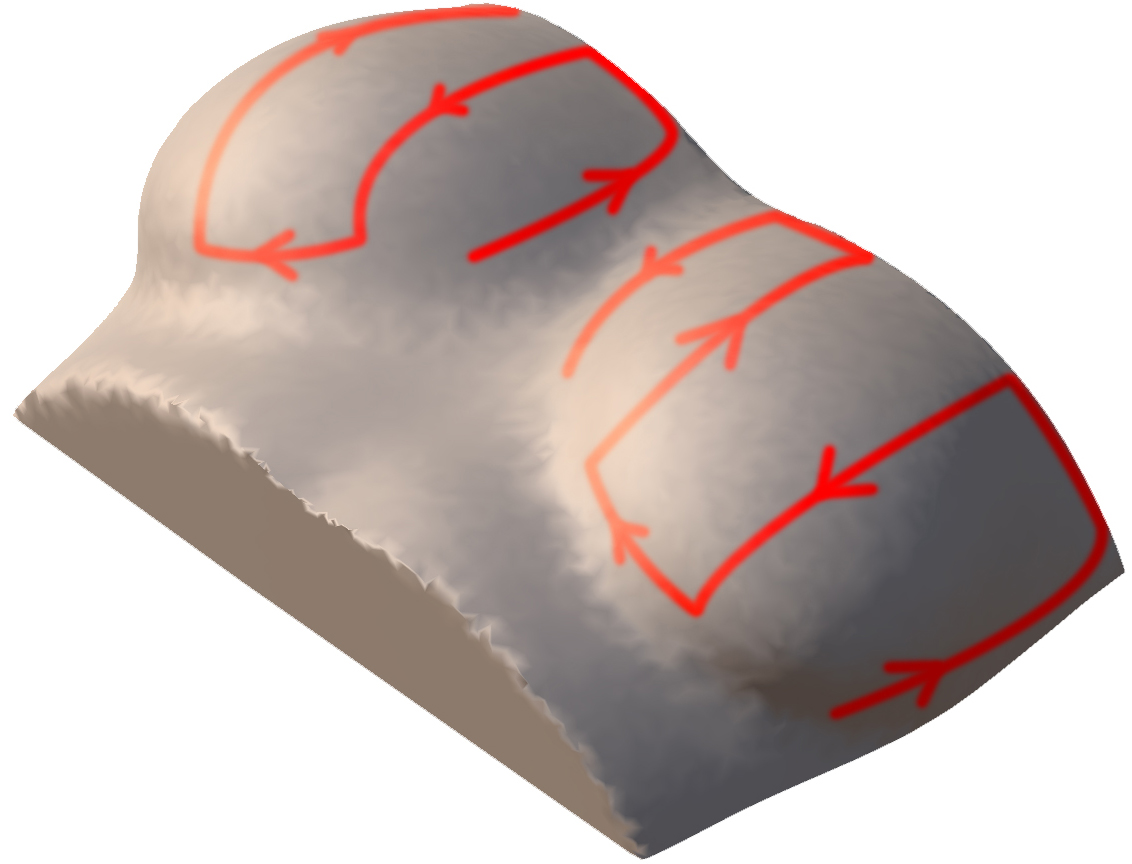
\includegraphics[width=0.75\textwidth]{figurer/d/probebevagelse}
    \caption{Det specifikke bevægelsesmønster ved scanning}
    \label{Probensbevagelse}
\end{figure}

Lars Bolvig tilføjede også, at Automatisk Ultralydsscanner skal kunne betjenes af radiografer. Så Automatisk Ultralydsscanner skal fungerer ved, at radiografen tager videoclipsne fra ultralydsscanningen og sender dem til radiologen, som bestemmer videre behandlingsforløb.

Se bilag \ref{Telefoninterview} Telefoninterviewet med radiolog Lars Bolvig. 

\section{Økonomisk og omkostningseffektiv analyse}
Formålet med denne analyse er at belyse det økonomiske perspektiv, ved at mammografiscreeningsprogrammet blev udvidet til at inkludere ultralydsscanninger. Den økonomiske analyse er udført ved at lave et overslag over forskellen på udgifterne, hvis en radiolog skulle udføre ultralydsscanningerne, versus indførsel og implementering af Automatisk Ultralydsscanner, hvor en radiograf udføre ultralydsscanningerne. Til at belyse konsekvenserne ved at udvide screeningsprogrammet er der søgt nationale og internationale litteratur om emnet. 

\subsection{Økonomiske konsekvenser ved udvidelse af screeningsprogrammet} 
Den økonomiske analyse er et overslag med udgangspunkt i en breakeven analyse. Efter interview med radiograf Tine Bisgaard og radiolog Lars Bolvig, blev det sandsynliggjort, at radiografer kan betjene Automatisk Ultralydsscanner, hvorefter videoclip fra ultralydsscanningen gennemses af en radiolog, samme procedure, som ved mammografi. 
Radiologer bruger i dag tid på at transportere sig til og fra scanningsstedet, når der skal scannes på patienter. Transporttid er derfor en vigtig variabel i breakeven analysen. Breakeven analysen tager udgangspunkt i, hvor mange ressourcer der kan flyttes fra en radiolog til en radiograf, ift. omkostningen relateret til implementeringen af Automatisk Ultralydsscanner, hvis screeningsprogrammet blev udvidet. 

Det er antaget, at radiologs gennemsnitlig løn er omkring 369 kr./timen, mens en radiografs gennemsnitlige løn er omkring 173 kr./timen \cite{Lon}. De samlede omkostning for anskaffelse af udstyret til opsætning af Automatisk Ultralydsscanner er fundet ved indsamling af priser fra forskellige hjemmesider (Se bilag \ref{Okonomi} Økonomi for flere oplysninger). De samlede faste omkostninger for fuld implementering inkluderer engangsudgifter for opsætning og oplæring af radiografer i anvendelse af Automatisk Ultralydsscanner. Den samlede pris for Automatisk Ultralydsscanner ligger omkring 219.305,64 kroner, de samlede udgifter kan ses i Tabel \ref{FasteOmkostninger}. 

\begin{table}[htb]
\centering
\begin{tabular}{ | l | l | p{1\textwidth} | }
\hline
\textbf{Beskrivelse af udgift} & \textbf{DKK} \\\hline
Engangsudgifter til afskrivning & 201.668,00 \\\hline
Opsætning & 10.759,00 \\\hline
Oplæring af radiografer & 6.768,00 \\\hline
I alt & 219.305,64 \\\hline
\end{tabular}
\caption{Samlede udgifter for Automatisk Ultralydsscanner}
\label{FasteOmkostninger}
\end{table}

Der er for begge scenarier blevet beregnet en pris for én ultralydsscanning. Prisen pr. scanning med Automatisk Ultralydsscanner er nogenlunde konstant, mens den varierer ved scenariet, hvor radiologen foretager ultralydsscanningen, priserne variere grundet forskellige transporttider for radiologen.  
Prisen for én scanning med Automatisk Ultralydsscanner er udregnet ved at antage, at det er en radiograf, der foretager forberedelse, 3D scanning og selve ultralydsscanningen, hvorefter en radiolog vil bruge omkring 10 minutter på at tjekke scanningen igennem for at se, om patienten skal til en yderligere scanning. Prisen for dette er beregnet til 110,64 kroner. 

Prisen for én ultralydsscanning ved scenariet, hvor en radiolog foretager ultralydsscaningen, er udregnet ved at antage, at det er en radiolog, der foretager både forberedelse, ultralydsscreening og transporttid på komme frem og tilbage til scanningsstedet. Hvis transport for radiologen er under fire minutter, er scenariet med Automatisk Ultralydsscanner dyrest. Automatisk Ultralydsscanner er derimod billigere hvis transporttid er over 4 minutter. Tabel \ref{Breakeven} beskriver transportminutter, pris for én ultralydsscanning udført af radiolog, og total antal scanninger udført, før før Automatisk Ultralydsscanner er betalt hjem. 

\begin{table}[htb]
\centering
\begin{tabular}{ | c | c | c | p{0.49\textwidth} | }
\hline
\textbf{Transporttid (min)} & \textbf{Pris per scanning (DKK)} & \textbf{Antal screeninger} \\\hline
5 & 116,89 & 35.052,51 \\\hline
8 & 135,34 & 8.873,09\\\hline
10 & 147,64 & 5.923,66\\\hline
15 & 178,39 & 3.235,19 \\\hline
20 & 209,14 & 2.225,25\\\hline
30 & 270,64 & 1.369,94\\\hline
45 & 362,89 & 868,95 \\\hline
60 & 455,14 & 636,26 \\\hline
\end{tabular}
\caption{Breakeven analyse for antal transportminutter}
\label{Breakeven}
\end{table}

Analysen er et overslag og ikke en nøje udført business case, da alle udregningerne er skøn. Analysen ville fremstå bedre, hvis der havde medvirket flere radiologer og radiografer til estimering af tider på ultralydsscanninger. Det er generelt forsøgt at prissætte udgifterne forbundet med indførslen af Automatisk Ultralydsscanner relativt højt for at undgå for mange uforudsete omkostninger. Hvis et hospital vil købe udstyret, vil priserne for opsætning måske være lavere, hvis man laver en indkøbsaftale. Beregningerne har ikke taget højde for, at radiologen udfører flere ultralydsscanninger for en transporttid. Transporttid må derfor ses som et gennemsnit pr. patient. Se 

Der bliver i Danmark udført omkring 270.000 mammografiundersøgelser om året, som en del af screeningsprogrammet \ref{esundhed}. Det betyder, at Automatisk Ultralydsscanner med en pris på 110,64 kroner pr. ultralydsscanning vil øge udgifterne til screeningsprogrammet med omkring 30 mio. kroner om året, men med yderligere omkostninger til vedligeholdelse på Automatisk Ultralydsscanner. 

\subsection{Andre konsekvenser af udvidelse af screeningsprogram} 
Det er forsøgt at undersøge, hvilke andre konsekvenser en udvidelse af screeningsprogrammet for kvinder mellem 50-69 vil medføre, hvor der i dag benyttes kun røntgen til at tage billeder af brystvævet. Til undersøgelsen er der anvendt national og international litteratur for at belyse, om tidlig detektering af brystkræft er rentabel og omkostningseffektiv, eller om screeningsforløbet er dyrere end fordelene. 

Generelt belyser studierne, at der er fordele og ulemper ved at lave en screeningsproces. Sundhedsstyrelsen fremhæver for og imod argumenter i deres invitation til screeningsprogrammet \ref{Argumenter}. Argumenterne for er, at det er et bedre at behandle brystkræft på et tidligere tidspunkt, og der reddes omkring 6 ud af 1.000 kvinder fra at dø. Argumenterne imod er, at 13 ud af 1.000 kvinder vil blive udsat for overdiagnosticering, og screeninger kan give falsk tryghed eller svulsterne er godartede. 

Overdiagnosticering undersøges i reviewet ”The benefits and harms of breast cancer screening: an independent review (2012)” \ref{Panel} fra Department of Epidemiology and Public Health. Reviewet betår af et uafhægigt panel med ekspertise i epidemilogi og medicinsk statistik, som undersøgte 11 RCT’s af screeninger for brystkræft, og deres relative risici. Panelet estimerede, at ud af 10.000 50-årige kvinder, vil 43 brystkræftsrelaterede dødsfald blive forhindret, mens 129 vil være overdiagnosticeret. Et Cochrane review har lavet en randomized controlled trial (RCT), som sammenligner to grupper, hvoraf den ene udsættes for mammografi screeninger. Forfatterne konkluderer, at screening reducerer brystkræft med 15\%, mens 30\% overdiagnosticeres og får overbehandling. Det betyder, at flere kvinder vil opleve at blive diagnosticeret, fordi de har gennemgået screeningen\ref{Gotzche}. 

Et BC Cancer review fra 2009 \ref{FyldigeBryster}  undersøgte, konsekvenserne af at scanne kvinder med fyldige bryster, hvor røntgen undersøgelsen var negativ, med ultralyd . Reviewet kunne ikke konkludere, om ultralyd som supplement er brugbart ved disse kvinder, men der var tre gange så mange kvinder, der fik lavet en biopsi ved ultralydsscanninger. Et japansk studie lavede en RCT, som undersøgte, hvorvidt man ved kombinationen af røntgen og ultralyd vil opdage flere kræfttilfælde. Studiet viste, at der ved kombinationen blev fundet flere typer 0 og I i interventionsgruppen, mens der ved stage II ikke var signifikant forskel. Studiet fandt også, at der var en højere rate af falsk-positive tilfælde ved at anvende ultralyd sammen med mammografi. 

Det amerikanske Cancer Society har estimeret overlevelsens procenten for en 5 årig plan, der er opdelt efter stadiet, kræften er i. Det er estimeret, at den relative overlevelsesprocent ved stadie 0 og 1 er tæt på 100 \%, stadie II har en relativ overlevelsesprocent på 93\%, stadie III har en på 72\% og stadie IV har en overlevelsesprocent på 22\% . 

Som pejlemærke til omkostningseffektiviteten kan benyttes kvalitet justeret leveår (QALY) til at beskrive, hvor rentabel en behandling er. I Danmark er der ikke en officiel grænse for, hvor meget én QALY bør koste, men Sundhedsstyrelsen har i en medicinsk teknologivurdering fra 2002 beskrevet: ”det kan anføres, at man generelt anser behandlinger, der koster mindre end 160.000 kr. pr. QALY for omkostningseffektive, mens behandlinger der koster mere end 800.000 kr. pr. QALY anses for ikke at være omkostningseffektive.\ref{QALY}”

Et spansk studie viste, at de inkrementielle omkostninger, når man gik fra ingen scanninger til en scanning hver andet år var 4,469 € per QALY, hvilket i danske kroner svarer til 33241,76 kroner per QALY. RCT'en ”Cost effectiveness of the NHS breast screening programme: life table model”  undersøger omkostningseffektiviteten af National Health Service (NHS), Englands sundhedsvæsen. Heri konkluderes det, at screening var forbundet med 2040 ekstra QALY med en ekstra omkostning på 45.5 mio. pund eller 20.800 per vunden QALY. Dette svarer i danske kroner til 183.335 per vunden QALY. 

Næsten alt den fundne litteratur drager konklusionen om, at mere forskning er nødvendig på området. Det kan derfor være svært at lave en endelig konklusion på, hvorvidt en udvidelse af screeningsforløbet vil være en god idé. Man kan forestille sig, at man ikke vil tilføje ultralydsscanninger til mammografiscreeningerne, da det øger chancen for overdiagnosticering, og det vil øge omkostningerne for både selve scanningen, behandlingen og de yderligere undersøgelser. 








\chapter{Medicinsk godkendelse}\label{MedicinskGodkendelse}
Den medicinske godkendelse er lavet for at undersøge, hvad der skal til, for at Automatisk Ultralydsscanner kan blive CE-mærket og derved godkendt til markedsføring i Europa. 

Medical Device Directive 93/42/EØF (MDD)\cite{MDD} er hoveddirektivet for medicinsk udstyr i Europa og danner grundlag for de godkendelsesprocedurer, der skal til, for at få medicinsk udstyr CE-mærket. Det er et lovkrav at overholde MDD, når man godkender medicinsk udstyr. MDD er indskrevet i dansk lovgivning ved bekendtgørelse om medicinsk udstyr \cite{Be}.
Alt kursiv i dette afsnit, er citater fra MDD.

\section{Definition}
Medicinsk udstyr er i MDD defineret som: 

\emph{»Medicinsk udstyr«: Ethvert instrument, apparat, udstyr, software, materiale eller anden genstand anvendt alene eller i kombination, herunder software, som af fabrikanten er beregnet til specifik anvendelse til diagnostiske eller terapeutiske formål, og som hører med til korrekt brug heraf, og som af fabrikanten er beregnet til anvendelse på mennesker med
henblik på:}
\let\labelitemi\labelitemii \emph{\begin{itemize}
\item diagnosticering, forebyggelse, overvågning, behandling eller lindring af sygdomme,
\item diagnosticering, overvågning, behandling, lindring af eller kompensation for skader eller handicap,
\item undersøgelse, udskiftning eller ændring af anatomien eller en fysiologisk proces, eller
\item svangerskabsforebyggelse,
\end{itemize}}
\emph{og hvis forventede hovedvirkning i eller på det menneskelige legeme ikke fremkaldes ad farmakologisk, immunologisk eller metabolisk vej, men hvis virkning kan understøttes ad denne vej.}

Med udgangspunkt i denne definition af medicinsk udstyr, går Automatisk Ultralydsscanner under kategorien som værende medicinsk udstyr. Dette begrundes med at Automatisk Ultralydsscanners primære opgave er automatiske ultralydsscanninger til srceening for brystkræft, og derved har til formål at forebygge af sygdomme. MDD skal derfor overholdes. 

\section{Klassificering}
Da Automatisk Ultralydsscanner er medicinsk udstyr, skal der foretages en klassificering af systemet. Klassificeringen foretages for at finde ud af hvilken procedure der skal anvendes for at få CE-mærket Automatisk Ultralydsscanner. Klassificeringen afspejler den risiko, der er forbundet med anvendelsen af udstyret. Jo højere klassificering, jo højere risiko er der ved anvendelsen af udstyret og jo længere er godkendelsesproceduren for CE-mærkningen. 
Klassificeringen er som følgende: 
\let\labelitemi\labelitemii \begin{itemize}
\item Klasse I - Udstyr med lav risiko for beskadigelse af bruger/patient. Inføres ofte ikke i kroppen.
\item Klasse IIa - Udstyr med reduceret risiko for beskadigelse af bruger/patient. Bruges kort tid og tilføres energi eller indføres i kroppen.  
\item Klasse IIb -  Udstyr med risiko med beskadigelse af bruger/patient. Bruges i længere tid og tilføres energi eller skal indføres i kroppen. 
\item Klasse III - Udstyr med høj risiko for beskadigelse af bruger/patient i tilfælde af fejl. F.eks hjerteklapper \cite{Delta}. 
\end{itemize} 

I MDD, er der 18 regler, man klassificerer medicinsk udstyr ud fra. 
Regel 10 omhandler aktive anordninger beregnet til diagnosticering og overvågning af vitale fysiologiske processer. Dette passer på Automatisk Ultralydsscanner, da det er et system, som er tilsluttet en ultralydsscanner, hvilket gør Automatisk Ultralydsscanner til en aktiv anordning.  

Citat fra MDD regel 10:  
\emph{Aktiv anordninger, der er beregner til diagnosticering, henhører under klasse IIa: - hvis de er beregnet til at muliggøre en direkte diagnosticering eller overvågning af vitale fysiologiske processer...}

Da Automatisk Ultralydsscanner er beregnet til overvågning af vitale fysiologiske processer og ikke skal bruges på patienter i længere tid, er Automatisk Ultralydsscanner klasse IIa. 

\section{CE-Mærkning}
Klassificering af Automatisk Ultralydsscanner danner grundlag for proceduren for CE-mærkning. 

Inden Automatisk Ultralydsscanner kan CE-mærkes, skal producenten igennem en række godkendelsesprocedurer. Definering og klassificering, som er gjort overfor, er en del af de procedure, producenten skal udføre. Derudover skal producenten overholde væsentlige krav fra MDD. Der skal udarbejdes teknisk dokumentation for produktet, bestående af en risikoanalyse og klinisk evaluering. Producenten skal ydermere lave et kvalitetssikringssystem og have et post market surveillance system, et system for hvordan producenten vil holde øje med produktet og andre lignende produkter, når det er kommet ud på markedet. Derudover skal producenten have en EF-overensstemmelseserklæring, hvor der  erklæres at produktet opfylder bekendtgørelsens krav \cite{Vej}. Når EF-overensstemmelseserklæring er underskrevet, kan producenten påføre CE-mærket. Som producent i Danmark, skal man registreres hos Lægemiddelstyrelsen, før markedsføringen kan påbegyndes. Producenten kan selv vælge et bemyndiget organ, som godkender, at producentens dokumentation lever op til gældende lovgivning. \cite{Klasse} 

Godkendelsesproceduren er et stort arbejde, da MDD er kompliceret at læse og forstå. Godkendelsesproceduren kan gøres lettere ved i stedet at følge en række standarder, som er harmoniseret i forhold til MDD. Til den medicinske godkendelse af Automatisk Ultralydsscanner er de harmoniserede standarder til risikohåndteringen DS/EN ISO 14971:2012 \cite{14971} og kvalitetssikring DS/EN ISO 13485:2012 \cite{13485} blevet anvendt. Se hvordan standarterne er anvendt nedenfor. 

\subsection{Risikohåndtering}
Da projektet er et undersøgelsesprojekt og udviklet for at teste muligheden for at udføre automatiserede ultralydsscanninger til screening for brystkræft. Og at udviklingsforløbet startede før der var kendskab til kravet om en risikohåndtering, er Automatisk Ultralydsscanner ikke udviklet med hensyn til risikohåndteringen. Der er dog stadig udført risikohåndtering på Automatisk Ultralydsscanner, hvor DS/EN ISO 14971:2012 \cite{14971} er blevet fuldt, for at vurdere risikoniveuet for Automatisk Ultralydsscanner som et færdigt produkt. 

I risikoanalysen blev der identificeret risici ved Automatisk Ultralydsscanner. De identificerede risici blev vurderet ved at se på sandsynlighed for at risicien ville opstå samt en konsekvens af at risicien opstod. Sandsynligheden blev vægtet fra 1-5, hvor 1 var meget usandsynlig og 5 var meget sandsynlig. Konsekvensen blev også vurderet fra 1-5, hvor 1 var ubetydelig og 5 var ødelæggende. Hver risici blev vurderet med en kombination af sandsynlighed og konsekvens. Se bilag \ref{Godkendelsesprocedure} Godkendelsesprocedure, for at se hvordan risici er identificeret samt hvordan risiciene er blevet analyseret. 

I risikoevalueringen blev risiciene indtaget i en risikomatrix, som tydeliggør kombinationen af sandsynligheden og konsekvensen. Risikomatrixen gør det let at overskue, hvilke risici som skal reduceres samt det samlede risikoniveau for Automatisk Ultralydsscanners.  

Tabel \ref{Niveau} viser risikomatrixens farvers betydning. 

\begin{figure}[H]
    \centering
    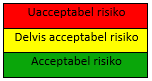
\includegraphics[width=0.25\textwidth]{figurer/r/Niveau}
    \caption{Risikomatrixens farvers betydning}
    \label{Niveau}
\end{figure}

Tabel \ref{Risiko} på næste side viser de fundne risici for Automatisk Ultralydsscanners samlet i en risikomatrix. Tallene i risikomatrixen henviser til de fundne risici fra risikoanalysen, se bilag \ref{Godkendelsesprocedure} Godkendelsesprocedure, afsnit om risikoanalyse.  

\begin{figure}[H]
    \centering
    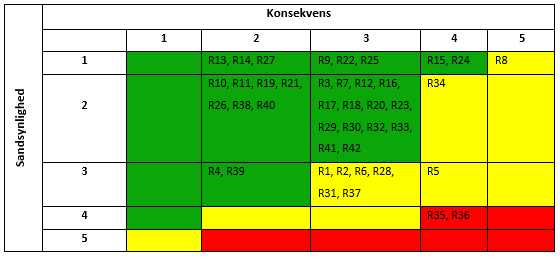
\includegraphics[width=1\textwidth]{figurer/r/Risiko}
    \caption{Risikomatrix}
    \label{Risiko}
\end{figure}

ISO 14971:2012 specificerer ikke hvad en acceptabel risiko er, men producenten er altid forpligtiget til at reducere risici mest muligt \cite{14971}. Ud fra risikomatrixen ligger Automatisk Ultralydsscanners samlede risikoniveau, i den acceptable ende, da der er flest risici i det grønne område. Risiko R35 – \textit{Kalibrering mellem robotarm og 3D kamera er forkert} og R36 - \textit{Bevægelsesmønster af robotarm er uhensigtsmæssigt}, ligger i det uacceptable niveau. Derfor bør der laves risikoreduktion på disse to risici, hvor muligheden for at mindske sandsynligheden for at risiciene vil opstå vurderes. Dette kunne f. eks ske ved at lave hyppige tests af systemet, oplæring af Operatør i hvordan Automatisk Ultralydsscanner kalibreres, samt en detaljeret beskrivelse af hvad et hensigtsmæssigt bevægelsesmønster, for Automatisk Ultralydsscanner er. Se bilag \ref{Godkendelsesprocedure} Godkendelsesprocedure, afsnit om Risikohåndtering for at se hvordan risikohåndteringen er foretaget. 

\subsection{kvalitetssikring}
Når man producere medicinsk udstyr, skal man også have et Kvalitetsstyringssystem (QMS). QMS dækker over en dokumenteret plan for, hvordan producenten sikrer at opfylde kravene specificeret i lovgivningen og kan opfyldes ved at følge ISO 13485:2012 \cite{13485}. Et QMS skal indeholde oplysninger om organisationen, ansvarsfordeling, arbejdsprocesser og procedure samt ressourcer der er til rådighed i produktionen. Derudover skal der være sporbarhed i alle dokumenter og komponenter der er anvendt i produktet, så man kan finde tilbage i produktet ved eventuelle fejl. \cite{13485}
Der er ikke udviklet et kvalitetssikringssytem over Automatisk Ultralydsscanner. Se bilag \ref {Godkendelsesprocedure} Godkendelsesprocedure, afsnit om Kvalitetssikring, hvor det beskrives hvordan et kvalitetssikringssystem kan udvikles. 

\section{Softwaregodkendelse}
Da Automatisk Ultralydsscanner har software, som styrer robotarmen, skal krav til medicinsk software også overholdes. Der er krav om en dokumenteret udviklingsproces, vedligeholdelsesplan, risikohåndtering og plan for løsning af softwarefejl. Standarden DS/EN 63204:2006 - Software for medicinsk udstyr - Livscyklusprocesser for software \cite{software} er anvendt, til at beskrive hvordan krav til medicinsk software kan overholdes. Se bilag \ref {Godkendelsesprocedure} Godkendelsesprocedure, afsnit om Softwaregodkendelse.

Den fulde medicinske godkendelse kan ses i bilag \ref {Godkendelsesprocedure} Godkendelsesprocedure.

\chapter{Systemarkitektur}\label{Systemarkitektur}
Der er udarbejdet forskellige diagrammer på baggrund af de specificerede systemkrav.  Diagrammerne har til formål at dele systemet op i realiserbare dele for at vise arkitekturen for systemet. 

Arkitekturen beskriver den grundlæggende organisering af Automatisk Ultralydsscanner og opbygningen af dens tilhørende PC Applikation. Systemet er opbygget generisk, så man vil kunne udskifte komponenter som f.eks. Robotarm eller 3D kamera med en anden type eller model. Udskiftning af komponenter vil dog resultere i en anderledes implementering. Der er i diagrammerne designet ud fra, at 3D kamera er af typen Microsoft Kinect 2.0 og Robotarm er en UR10 robot. 

\section{Systemoversigt}
Systemet Automatisk Ultralydsscanner består af en PC applikation, en Ultralydsscanner, en Robotarm af typen Universal Robots UR10, et 3D kamera af typen Microsoft Kinect 2.0, samt et Access Point, af typen D-Link DAP-1160, til forbindelse mellem Robotarm og PC applikation. Der er fem aktører, Robotarm, Ultralydsscanner, 3D kamera, Operatør og Patient, som interagerer med PC Applikation.

Robotarm har en touch skærm, hvorpå Operatør manuelt kan flytte Robotarm, se Robotarms koordinator samt programmere Robotarm. Robotarm er forbundet via et ethernet kabel af typen RJ45 til et Access Point. PC Applikation er forbundet til Access Point med et kabel af samme type. 3D kamera er forbundet til PC Applikation via 3D kameras USB 3.0 kabel. Ultralydsscanner er en seperat enhed, som blot er fastgjort mekanisk på Robotarms yderste led, men indgår i det fulde system Automatisk Ultralydsscanner. Ultralydsscanner skal manuelt tændes og slukkes af Operatør.

For Automatisk Ultralydsscanner er der udarbejdet forskellige diagrammer, som har til formål at dele systemet op i blokke og vise integration mellem blokkene, samt forbindelser mellem aktører. Diagrammerne vil blive gennemgået nedenfor. 
\newpage

\subsection{Domænemodel}
Domænemodellen på Figur \ref{domain} viser forbindelserne mellem de forskellige aktører i systemet. 

\begin{figure}[H]
    \centering
    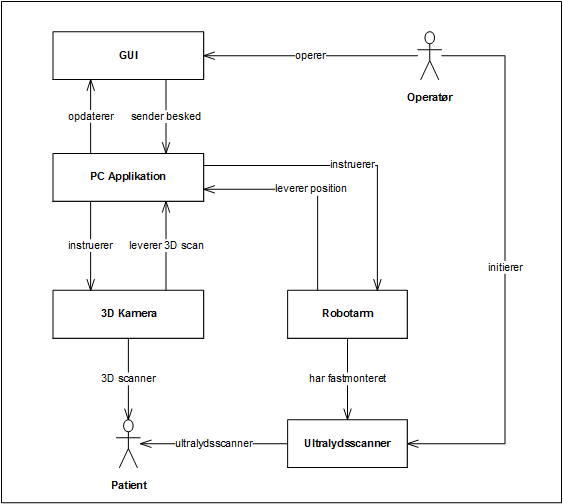
\includegraphics[width=0.7\textwidth]{figurer/d/Design/uml_domain}
    \caption{Domænemodel for Automatisk Ultralydsscanner}
    \label{domain}
\end{figure}

\subsection{Block Definition Diagram}
Block Definition Diagram Figur \ref{BDD} giver et overblik over Automatisk Ultralydsscanners komponenter, som et samlet system.
Her ses, at det er nødvendigt at have en computer med mus og skærm for at anvende PC Applikation.

\begin{figure}[H]
    \centering
    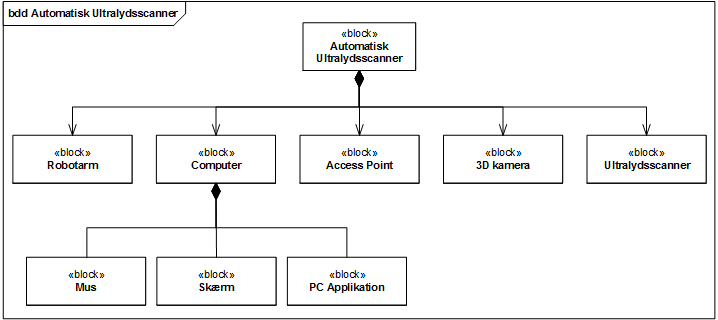
\includegraphics[width=1\textwidth]{figurer/d/Design/BDD}
    \caption{BDD for Automatisk Ultralydsscanner}
    \label{BDD}
\end{figure}
\newpage

\subsection{Internal Block Diagram}
Internal Block Diagram Figur \ref{IBD} viser flow af information mellem de forskellige blokke i Automatisk Ultralydsscanner.
Bemærk at Ultralydsscanner ikke er med, da den ikke interagerer med resten af Automatisk Ultralydsscanner, men blot er forbundet mekanisk til Robotarm.
Når 3D Scan menuen åbnes i PC Applikation, vil der være et konstant flow af dybdedata fra 3D kamera til PC Applikation.
Når PC Applikation startes, vil der være et flow af data frem og tilbage mellem Robotarm og PC Applikation, hvor Access Point agerer som mellemled. 
Forbindelsen mellem PC Applikation og Access Point, samt forbindelsen mellem Access Point og Robotarm er oprettet med ethernet-kabler af typen RJ45.
Forbindelsen mellem PC Applikation og 3D kamera er oprettet med 3D kameras USB 3.0 kabel. 

\begin{figure}[H]
    \centering
    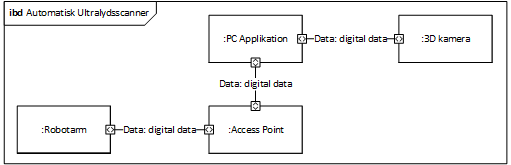
\includegraphics[width=1\textwidth]{figurer/d/Design/IBD}
    \caption{IBD for Automatisk Ultralydsscanner}
    \label{IBD}
\end{figure}

\section{Systemets grænseflader}
Systemet består af to grænseflader: Mellem PC Applikation og Kinect, og mellem PC Aplikation og UR10. Kommunikationen mellem PC Applikation og UR10 sker over modbus-protokollen, hvor kommunikationen mellem PC Applikation og Kinect er gennem Kinect's API.

\subsection{UR10}
Overførsel af data til UR10 sker gennem Transmission Control Protocol/IP-protokollen (TCP/IP). Til afsendelse af positur-værdier fra PC Applikation anvendes modbus-protokollen. Modbus-protokollen sørger for at skrive binære værdier på registre på UR10-controlleren. UR10 kører på URScripts, hvis den skal styres automatisk. UR10 har et script der i en uendelig løkke læser værdierne på registrene og instruerer UR10s Tool Center Point (TCP) til at flytte sig til en positur med en given acceleration og hastighed.

\subsubsection{TCP/IP}
PC Applikation skriver til UR10 over en TCP/IP forbindelse på en IP. Der anvendes to porte; port 502 for kommunikation over modbus-protokollen, og port 30002 for indlæsning af nuværende værdier.
Kommunikationen over port 502 er både read og write, hvor port 30002 kun er read. 
Bemærk, at forskellen  ligger i at de værdier der bliver overført på port 502 kun er til styring af UR10 på script-niveau, som fx den ønskede positur, hastighed og acceleration. Modsat, på port 30002, indhentes de nuværende tilstandsværdier som UR10 har, som fx posituren den reélt har, som ikke nødvendigvis er den samme som den sidste ønskede positur.
For at give et eksempel på hvordan dette foregår sekvensmæssigt:
PC Applikation sender en positur over port 502. Værdierne i denne positur indskrives på UR10s registre.
URScriptet aflæser disse værdier og instruerer UR10 i at flytte sit TCP til denne positur.
Efter noget tid vil den have nået denne positur. Der vil løbende kunne aflæses om UR10 har nået posituren på port 30002.

\textbf{Port 502}
Skriv tekst

\textbf{URScript}
Scriptet der kører på UR10 aflæser i alt 3 værdier:
Acceleration, hastighed og positur.
Positur består af værdierne X, Y og Z for position og RX, RY og RZ for rotation.
Positur-værdierne aflæses på registrene 135-140 og indsættes som properties i et 'pose' objekt.
Accelerationsværdien, hastighedsværdien samt pose-objektet gives som parameter til funktionen \textit{movel}.
UR10s TCP flyttes lineært i funktionen \textit{move1}. Tiden på acceleration og deceleration styres omvendt proportionalt af accelerationsværdien, mens den maksimale hastighed styres af hastighedsværdien.

\textbf{Port 30002}
Der er mulighed for at hive informationer om stort set alle robottens nuværende tilstande som fx software version, ledrotationshastighed, tryk feedback m.m. I implementeringen anvendes der kun TCPs rotation og position.

\subsection{Kinect}
Computeren er forbundet til 3D kamera via USB af typen Transcend PDU3 USB-adapter PCIe 2.0 USB 3.0 eller anden USB3.0 type, der er kompatible med Microsoft Kinect 2.0. 3D kamera har også et supplerende strømforsyningskabel.
For kommunikation med 3D kamera er der brugt Microsoft's Kinect API \cite{KinectAPI} .
Der er taget udgangspunkt i Fusion-delen \cite{KinectFusion} af API'et. Fordelen med dette API er at det kan gøre en masse arbejde - ulempen er at det ikke er generisk. Altså ville man ikke kunne bruge en anden sensor en Microsoft Kinect for Windows 2.0. API'et har en C\#-wrapper, og Microsoft har leveret kildekode til et projekt der gjorde nogenlunde det vi var interesserede i (se reference \cite{KinectFusionExplorer} for at få den nyeste version af dette.
Efter oprettelsen af forbindelse til Kinect sensoren er det muligt at 'lytte' på den og få de depth frames den kontinuerligt leverer. Se beskrivelsen af klassen KinectFusionizer underafsnittet \ref{ComputerVisionLibrary}  ComputerVisionLibrary. 

\newpage

\section{Softwarearkitektur}
PC Applikation er opdelt af forskellige moduler for at øge samhørigheden og nedsætte koblingen, hvilket er med til at sikre overskuelighed og gøre PC Applikation lettere at vedligeholde og genbruge. Modulerne er inddelt efter ansvarsområder angående præsentation til bruger, kommunikation til Robotarm, indhentning af 3D scan fra 3D kamera samt udregning af Robotarms sti til ultralydsscanning. Disse 4 moduler har fælles datastrukturer. For at undgå cykliske forbindelser, er disse datastrukturer tilføjet til deres eget modul. Figur \ref{Layers} viser referencen mellem modulerne. 

\begin{figure}[H]
    \centering
    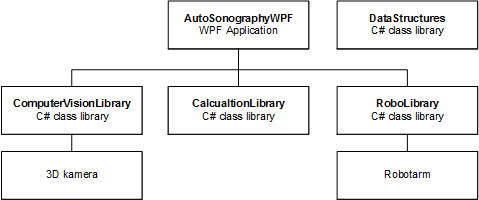
\includegraphics[width=0.75\textwidth]{figurer/d/Design/Layers}
    \caption{PC Applikations opdeling af moduler}
    \label{Layers}
\end{figure}


\begin{table}[htb]
\begin{tabular}{ | l | p{0.7\textwidth} | }
\hline
\textbf{Lag} & \textbf{Beskrivelse af ansvar} \\\hline
AutoSonographyWPF & Håndterer Operatørs interaktion med PC Applikation, hvor Operatør kan vælge 3D scan- eller ultralydsscan. Dette projekt virker som en grænseflade til resten af PC Applikation.\\\hline
ComputerVisionLibrary & Indhenter og afgrænser 3D scanning fra 3D kamera. \\\hline
CalculationLibrary & Sørger for at konvertere en 3D scanning til en sti af positurer som Robotarm kan gennemløbe. \\\hline
RoboLibrary & Muliggør at kommunikere med og instruere Robotarm.\\\hline
DataStructures & Indeholder forskellige data transfer objekter (DTO), der bruges gennem PC Applikation til at sende objekter mellem de forsellige moduler, samt udvidelsesmetoder til eksisterende .NET eller KinectAPI datastrukturer.\\\hline
\end{tabular}
\caption{Modulopdeling og ansvar}
\end{table}

\newpage
\subsection{Pakkediagram}
Pakkediagrammet figur \ref{Pakkediagram} giver en oversigt over afhængighederne i PC Applikation.
For at undgå cykliske forbindelser blev adskillige datastrukturer flyttet fra CalculationLibrary, ComputerVisionLibrary og RoboLibrary til DataStructures-biblioteket.
DataStructures indeholder altså kun nogle datastrukturer og nogle extension-metoder til disse. 
For forklaringen af indholdet af de øvrige pakker, se klassediagrammerne for hvert bibliotek.

\textbf{AutoSocograophyWPF} inderholder alt, der hører til PC Applikations grafiske brugergrænseflade (GUI).

\textbf{ComputerVisionLibrary} indeholder klasser, der interagerer med 3D kamera og udvinder en 3D scanning i et begrænset område.

\textbf{RoboLibray} indeholder klasser som der muliggør kommunikation med Robotarm. 

\textbf{DataStructures} indeholder datastrukturer der bruges på tværs af PC Applikation og nogle extension-metoder til disse. 

\textbf{CalculationLibrary} indeholder klasser der finder stien af positurer i en 3D scanning der er nødvendige for at foretage en ultralydsscanning med Robotarm.

\begin{figure}[H]
    \centering
    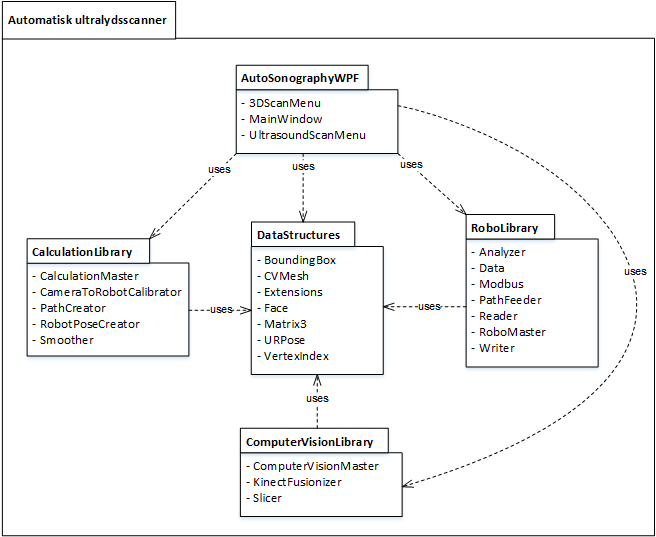
\includegraphics[width=0.9\textwidth]{figurer/d/Design/Pakkediagram}
    \caption{Pakkediagram for Automatisk Ultralydsscanner}
    \label{Pakkediagram}
\end{figure}
\newpage

\chapter{Systemdesign}\label{Systemdesign}
Der er udarbejdet forskellige diagrammer på baggrund af de specificerede systemkrav.  Diagrammerne har til formål at dele systemet op i realiserbare dele for at vise designet af systemet. 

\section{Pakkediagram}
Pakkediagrammet figur \ref{Pakkediagram} giver en oversigt over afhængighederne i PC Applikation.
For at slippe for cykliske forbindelser blev mange datastrukturer flyttet fra CalculationLibrary, ComputerVisionLibrary og RoboLibrary til DataStructures-biblioteket.
DataStructures indeholder altså kun nogle datastrukturer og nogle extension-metoder til disse. 
For forklaringen af indholdet af de øvrige pakker, se klassediagrammerne for hvert bibliotek.

AutoSocograophyWPF inderholder alt, der hører til Grafisk brugergrænseflade (GUI), herunder de tre menuer, 3DscanMenu, StartMenu og UltrasoundMenu. 

ComputerVisionLibrary indeholder klasser, der har at gøre med 3D billedet og konvetering til et mesh, herunder ComputerVisionMaster, KinectsFusionizer og PLYExporter. 

RoboLibray pakken indeholder klasser som robotarmen skal benytte for at kunne flytte sig, herunder Analyzer, Data, Logic, Modbus, PathCreator, PathFeeder, Reader, RoboMaster, URPose og Writer. 

DataStructures

CalculationLibrary

\begin{figure}[H]
    \centering
    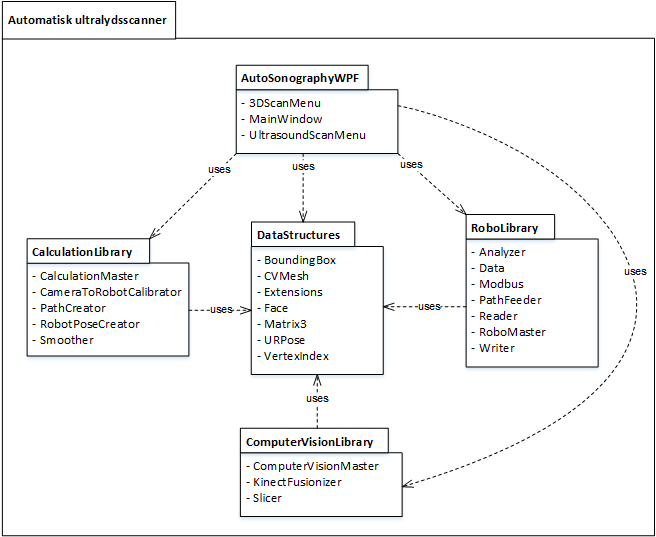
\includegraphics[width=1\textwidth]{figurer/d/Design/Pakkediagram}
    \caption{Pakkediagram for Automatisk Ultralydsscanner}
    \label{Pakkediagram}
\end{figure}
\newpage

\section{Klassediagram}
Dette afsnit beskriver klasserne fra pakkediagrammet. Klassediagrammerne viser strukturen i systemet og deres relationer. Hver klasse indeholder de vigtigste metoder og attributer i klassen, der udgør funktionaliteten i PC Applikation. 

\subsection{GUI}
Denne klasse indeholder brugergrænsefladen af PC Applikation.

\let\labelitemi\labelitemii
\begin{itemize}
\item{MainWindow}\newline
Giver anledning til at foretage et 3D scan. Såfremt en 3D scanning er gennemført giver det også anledning til at starte en ultralydsscanning.
Når menuen startes, oprettes en instans af RoboMaster, for at sætte Robotarm i standard positur. Dette er nødvendigt, hvis Robotarm skulle være i vejen for en 3D scanning.
Hvis der ikke er nogen forbindelse til Robotarm vil der 

\item{3DScanMenu}\newline
I denne menu er der mulighed for at se det nuværende dybdebillede, afgrænse området der skal 3D scannes og foretage en 3D scanning.

\item{UltrasoundScanMenu}\newline
I denne menu kan den procentvise færdiggørelse af ultralydsscanningen følges. Der er også mulighed for at pause samt afbryde ultralydsscanningsprocessen.
\end{itemize}

\begin{figure}[H]
    \centering
    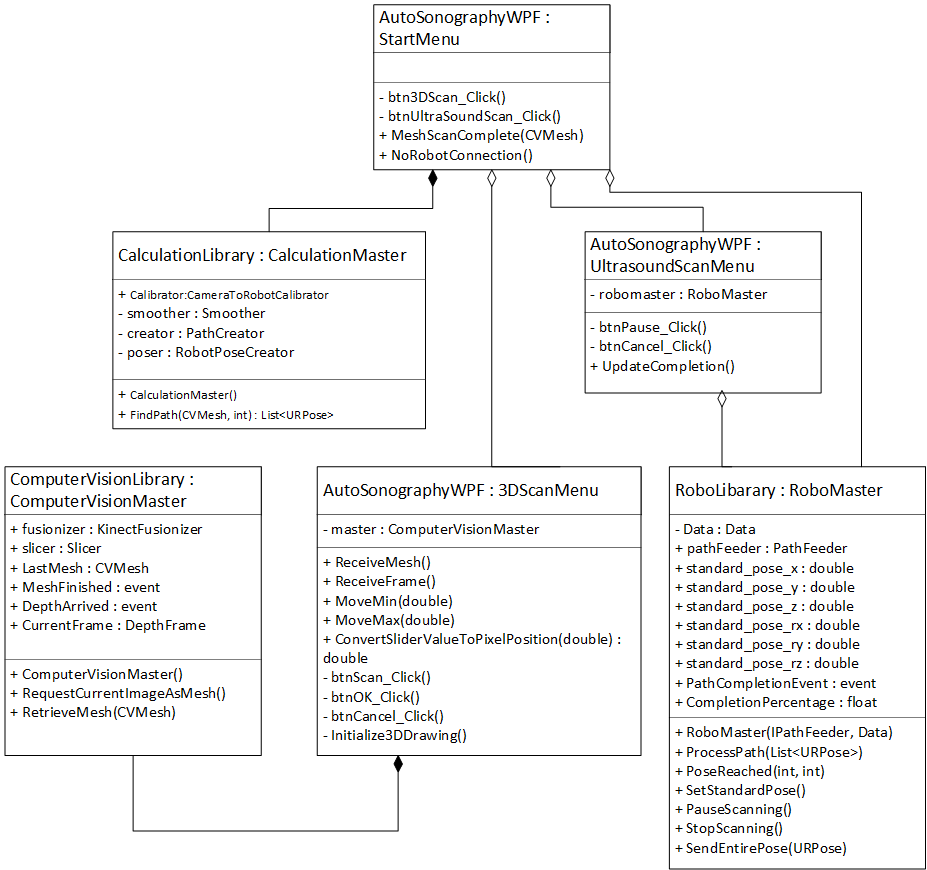
\includegraphics[width=1\textwidth]{figurer/d/Design/Class/uml_class_gui}
    \caption{Klassediagram for GUI}
    \label{class_gui}
\end{figure}
\newpage

\subsection{ComputerVisionLibrary}
Formålet med dette bibliotek er at få en afgrænset 3D scanning fra et 3D kamera.

\begin{itemize}
\item{KinectFusionizeren}\newline
Har til ansvar at åbne Kinect-sensoren, tage det nuværende dybdebillede fra sensoren og konvertere det til en mesh.

\item{ComputerVisionMaster}\newline
Denne klasse virker som den logiske grænseflade til KinectFusionizeren, hvor instansen af den nuværende mesh lagres her.
Andre klasser kan subscribe til ComputerVisionMasteren for at høre hvornår der er en ny mesh tilgængelig.

\item{Slicer}\newline
Denne klasse sørger for at fjerne de punkter i en mesh der er uinteressante:
\begin{enumerate}
\item{Faces der peger nedaf, dvs fejlpunkter. Da 3D kameraet er monteret i loftet, vil den ikke kunne se undersiden af det den skanner.}
\item{Duplikerede punkter. KinectFusionizer outputter punkter der er ens. Disse fjernes af optimeringsårsager.}
\item{Punkter og faces der er uden for det område der ønskes skannet. Dette inkluderer nærtliggende objekter som fx en væg, eller områder på patienten der ikke ønskes skannet.}
\end{enumerate}
\end{itemize}

\begin{figure}[H]
    \centering
    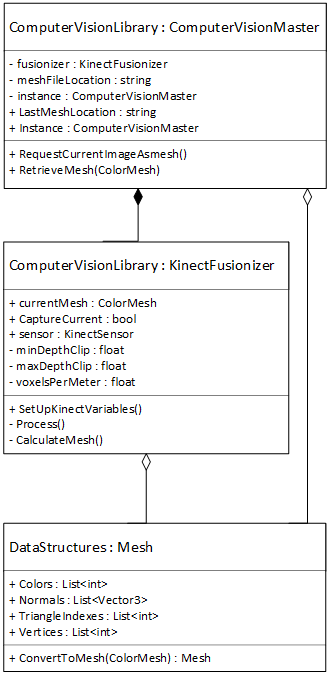
\includegraphics[width=1\textwidth]{figurer/d/Design/Class/uml_class_computervisionlibrary}
    \caption{Klassediagram for ComputerVisionLibrary}
    \label{class_ComputerVisionLib}
\end{figure}
\newpage

\subsection{CalculationLibrary}
Dette bibliotek agerer som bindeledet mellem ComputerVisionLibrary og RoboLibrary.

\begin{itemize}
\item{CameraToRobotCalibrator} \newline
Sørger for at konvertere 3D scanningen givet fra ComputerVisionLibrary fra 3D Kameras rum til Robot Arms rum.
Dette sker ved en kæde af matrix-transformationer i en speciel rækkefølge. 
Normaltvis har man en translation, rotation og skalering, men da Robot Arms og 3D Kameras koordinatsystemer begge er angivet i millimeter, er skaleringen unødvendig.
I tilfældet for dette projekt sker der først en rotering og derefter en translation, for at bestemme transformationsmatricen. 
Hvert punkt i en mesh konverteres så til det nye space. Se bilag \ref{RumTransformation} for inspirationen til denne klasse.

\item{Smoother}\newline
Denne klasse har til ansvar at udjævne en mesh. Med udjævning forstås at 'ensforme' normalerne, altså retningsvektorer i en mesh's faces.
Dette er nødvendigt da 3D Kameras output kan være uperfekt og dermed vil normalerne være ekstreme/deforme. Udjævningen sker gennem laplacian smoothing, se \cite{Smooth} for forklaring af algoritme.

\item{PathCreator}\newline
Klassen afgør listen af punkter i en mesh som der skal findes positurer til Robot Arm ud fra.
For at afgøre stien genereres der en 'bølge' - i implementeringen en squarewave - af punkter der draves over meshen.
De vertices i meshen der tilnærmer sig punkterne i bølgen bedst vil blive udvalgt til stien.

\item{RobotPoseCreator}\newline
I denne klasse vil konverteringen af en mesh-sti til en liste af positurer ske.
For hvert punkt i mesh-stien, vil en vertex' normal findes. 
Ved hjælp af normalen, sti-punktets koordinater samt længden på Robotarms probe kan den forskudte Robot Arm position findes.
Inverteres denne normal, kan det ses som en retningsvektor for en Robotarm.
Retningsvektoren konverteres først til en roll, pitch og yaw - altså roteringer omkring de tre retningsakser; X, Y og Z.
Da man ikke kan afgøre alle tre værdier ud fra en retningsvektor alene, sættes pitch til 0, da det er muligt at 'pege' et vilkårligt sted med en roll-rotering og en yaw-rotering. Disse værdier konverteres herefter til en rotationsvektor.
Positionsvektoren og rotationsvektoren udgør til sammen en positur, som tilføjes til listen af positurer. Matematikken for udregningen af rotationen kan ses på næste side.
\newpage

Givet en tredimensionel retningsvektor med en længde på 1
$$
v_{direction} = (X, Y, Z)
$$
Find de tre rotationer om de tre forskellige akser. Med en retningsvektor alene kan én af disse rotationer ikke findes. Da man vil kunne pege i en vilkårlig retning med en roll-rotering og en yaw-rotering, er pitch sat til 0.
$$ 
roll = acos(Z) \qquad 
pitch = 0 \qquad 
yaw = \begin{cases} 
	-acos(-Y) & X \leq 0\\
	acos(-Y)  & X > 0 \\
\end{cases}
$$

Opstil matricerne der skal bruges for at konvertere roll, pitch og yaw til en rotationsvektor.
%%%%%%%%%%%%%%%%%%%%
% Matricerne 
$$ 
Roll_M = \begin{bmatrix}
    1 & 0 & 0 \\
    0 & cos(roll) & -sin(roll) \\
    0 & sin(roll) & cos(roll)
\end{bmatrix}
\quad
Pitch_M = \begin{bmatrix}
    cos(pitch) & 0 & sin(pitch) \\
    0 & 1 & 0 \\
    -sin(pitch) & 0 & cos(pitch)
\end{bmatrix} 
$$
$$
Yaw_M = \begin{bmatrix}
    cos(yaw) & -sin(yaw) & 0 \\
    sin(yaw) & cos(yaw) & 0 \\
    0 & 0 & 1
\end{bmatrix}
$$ 

Ordnen af rotationerne er vigtig, derfor vil der først foregå en roll rotering, en pitch rotering og til sidst en yaw rotering. Prikken mellem matricerne her er dot-produktet.
$$\mathbb{R} = Yaw_M \cdot Pitch_M \cdot Roll_M $$

Dernæst kan $\theta$ og $\mu$ findes, der bruges til beregningen af $r_x$, $r_y$ samt $r_z$, der samlet udgør den endelige rotationsvektor $v_{rotation}$.

$$\theta = acos\bigg(\frac{\mathbb{R}_{0,0}+\mathbb{R}_{1,1}+\mathbb{R}_{2,2}-1}{2}\bigg) \qquad \mu = \frac{1}{2 \times sin(\theta)}$$

$$r_x =\mu \times(\mathbb{R}_{2,1}-\mathbb{R}_{1,2}) \times\theta $$
$$r_y =\mu \times(\mathbb{R}_{0,2}-\mathbb{R}_{2,0}) \times\theta $$
$$r_z =\mu \times(\mathbb{R}_{1,0}-\mathbb{R}_{0,1}) \times\theta $$
$$v_{rotation} = (r_x, r_y, r_z)$$

\end{itemize}

\begin{figure}[H]
    \centering
    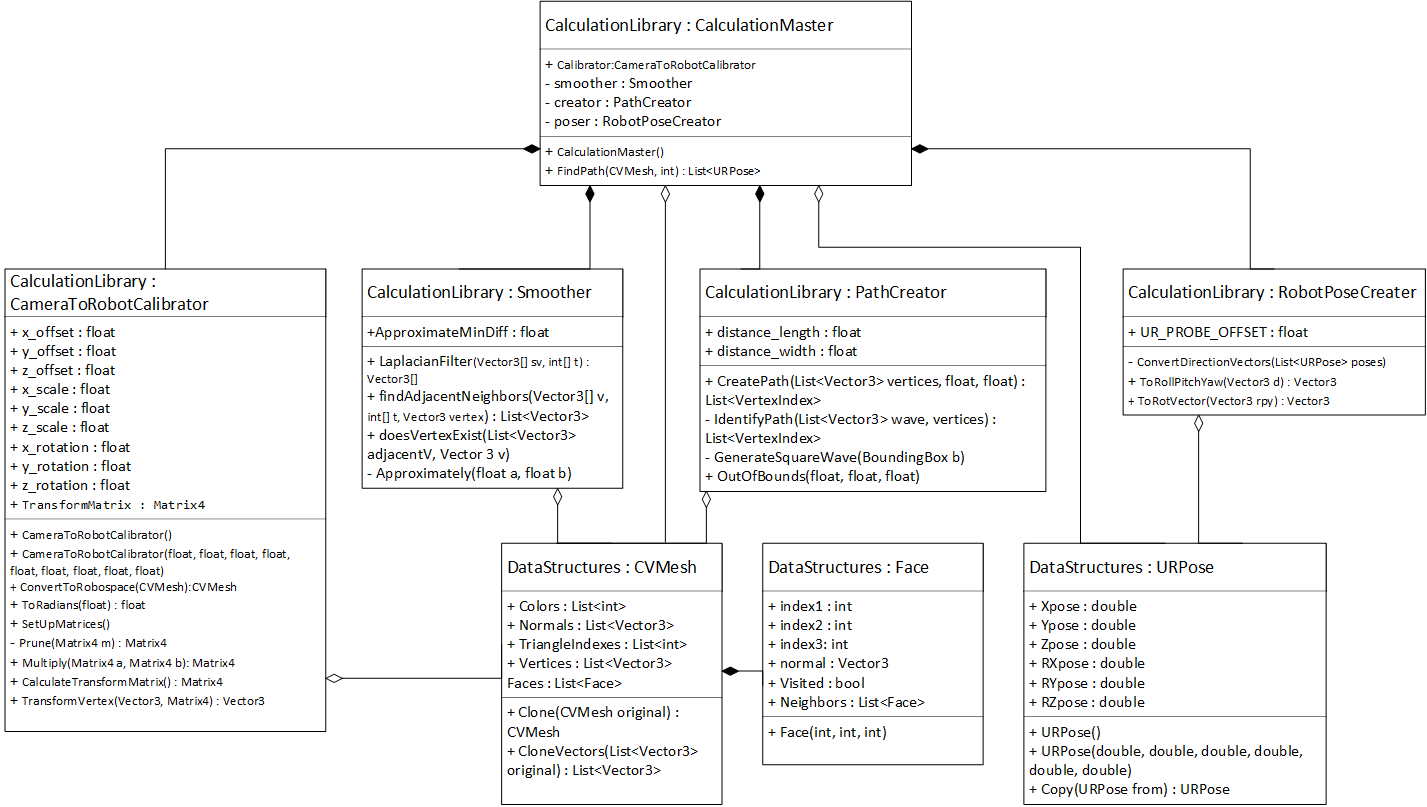
\includegraphics[width=1\textwidth]{figurer/d/Design/Class/uml_class_calculationlibrary}
    \caption{Klassediagram for CalculationLibrary}
    \label{class_ConversionLib}
\end{figure}
\newpage

\subsection{RoboLibrary}
Biblioteket giver mulighed for kommunikation med Robot Arm.

\begin{itemize}
\item{RoboMaster}\newline
Klassen agerer som bindeled mellem de øvrige klasser i biblioteket og GUI.

\item{PathFeeder} \newline
Står for at gennemløbe hver positur i listen, og kommunikere med Data for at finde ud af hvornår den næste positur skal sendes til Robot Arm.

\item{Data}\newline
Klassen virker som en grænseflade mellem den 'logiske' del af biblioteket og dens underliggende reader/writer klasser.

\item{Reader}\newline
Denne klasse står for kontinuerligt at læse data fra Robot Arm, for at afgøre dens nuværende positur. 

\item{Analyzer} \newline
Klassen konverterer det indlæste data til en objekt-orienteret model, altså transformation af bytes til Robot Arms nuværende positur.

\item{Writer}\newline
Klassen har til ansvar at omskrive værdier til binær data. Den omskriver både positurer samt konfigurationer.

\item{Modbus}\newline
Denne klasse skriver binær data ud på Robot Arms IP gennem modbus-protokollen.
\end{itemize}

\begin{figure}[H]
    \centering
    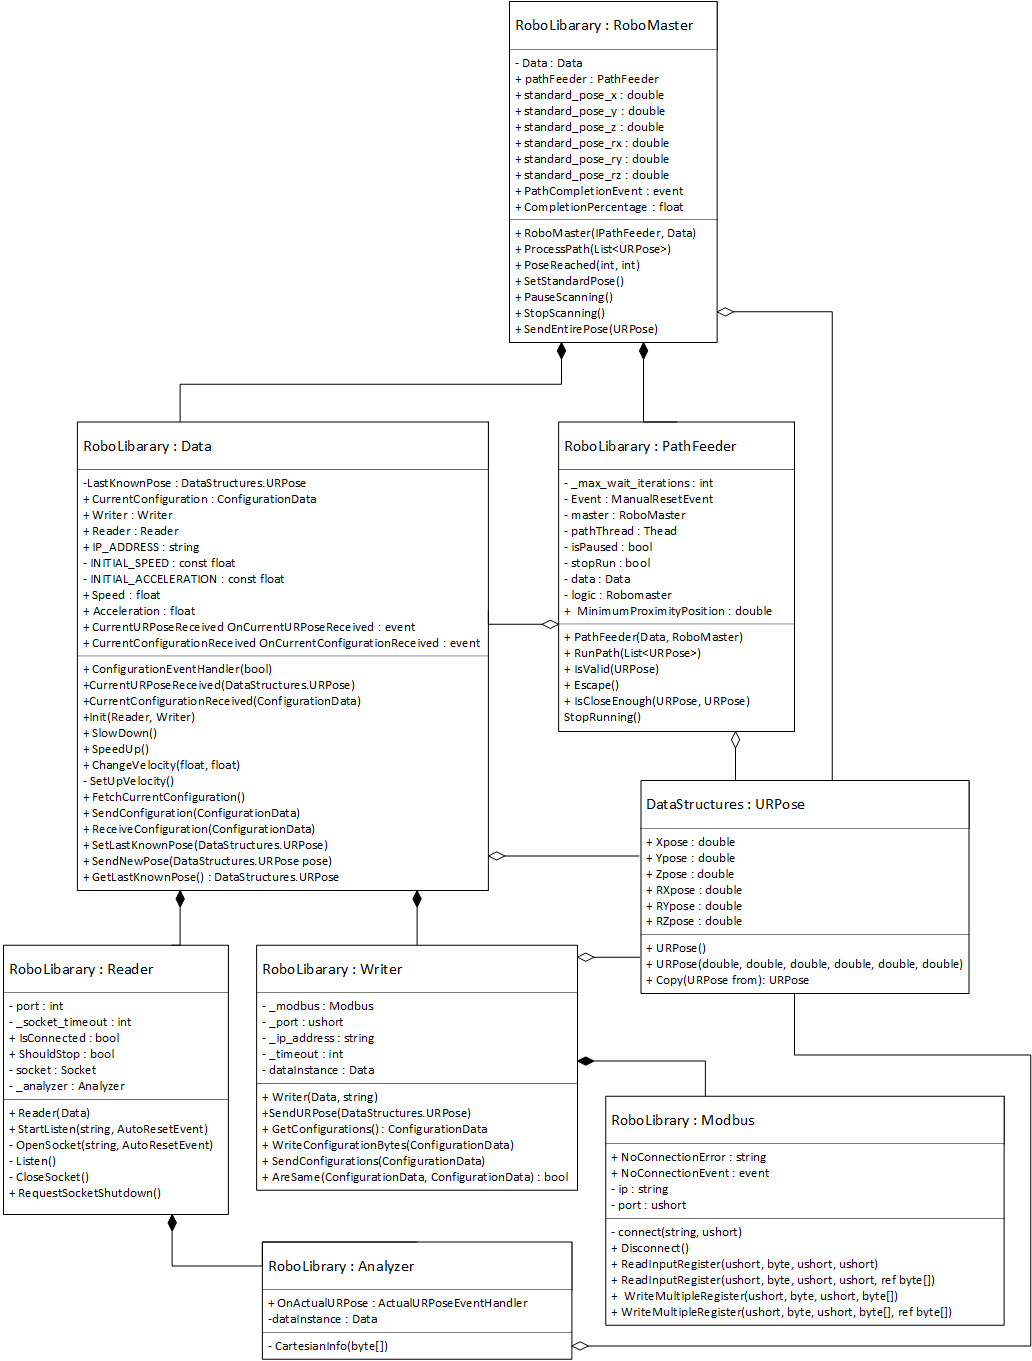
\includegraphics[width=1\textwidth]{figurer/d/Design/Class/uml_class_robolibrary}
    \caption{Klassediagram for RoboLibrary}
    \label{class_RoboLib}
\end{figure}

\newpage
\section{Sekvensdiagrammer}
Der er på baggrund af klassediagrammerne lavet sekvensdiagrammer, som beskriver systemets funktionalitet, og hvor de vigtigse metoder og attributter imellem klasserne er identificeret.

Nedenstående sektioner vil beskrive de vigtigste sekvensdiagrammer i system og fremvise, hvordan klasserne indbyrdes kommunikerer. 

\subsection{Read Robot Data} 
Reader initieres med en IP hvor den skal lytte på. 
Der åbnes en socket på denne IP, og derefter lytter den kontinuert i en baggrundstråd. 
Readeren giver de rå data videre til Analyzer som konverterer dem til Robot Arms nuværende positur.

\begin{figure}[H]
    \centering
    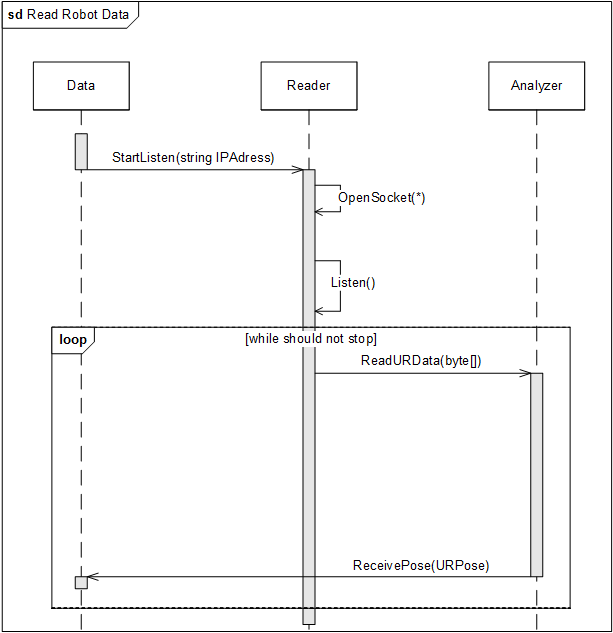
\includegraphics[width=1\textwidth]{figurer/d/Design/Sequence/sd_reading}
    \caption{Sekvensdiagram for Read Robot Data - indlæsning af Robotarms positur}
    \label{sd_reading}
\end{figure}

\subsection{3D scan}
Ved scan vil KinectFusionizeren stå for at tage et dybdebillede fra Kinect-sensoren.
Den vil dernæst konvertere dybdebilledet til en point cloud.Dette trianguleres, så der fås en mesh der efterfølgende kan bearbejdes. 3DScanMenu modtager meshen gennem event-kommunikation.
Gennem de beskræringsparametre der er valgt i menuen vil meshen dernæst beskæres i Slicer, så kun det ønskede område fremkommer. Efter beskæringen vises meshen som en rotérbar 3D model i menuen.

\begin{figure}[H]
    \centering
    \includegraphics[width=1\textwidth]{figurer/d/Design/Sequence/sd_3Dscan}
    \caption{Sekvensdiagram for 3D scan}
    \label{sd_3Dscan}
\end{figure}
\newpage

\subsection{Feed Path}
Efter konvertering af mesh output til robot positur sti, vil listen af positurer sendes fra RoboMaster til PathFeeder. 
Se sekvensdiagrammet 'Path Creation' for en gennemgang af hvordan disse positurer findes.
PathFeeder gennemløber hver positur og sender den næste i listen til Data, som videregiver posituren til Writer.
RoboMaster informeres løbende om hvor langt PathFeeder er med at gennemløbe punkter.
Writer konverterer posituren til binær data, og ModBus skriver dataen ud på Robot Arms register.
Hernæst ser PathFeeder på om Robot Arms nuværende positur har nærmet sig den ønskede positur. 
Når den er tæt nok på, hoppes der ud af 'while'-løkken, og den næste positur kan sendes.
Den Alt der er her skal forstås som at PathFeeder kører i sin egen baggrundstråd der kan pauses. 
Ved terminering af denne baggrundstråd vil PathFeeder stoppe med at videregive nye positurer til Robot Arm.

\begin{figure}[H]
    \centering
    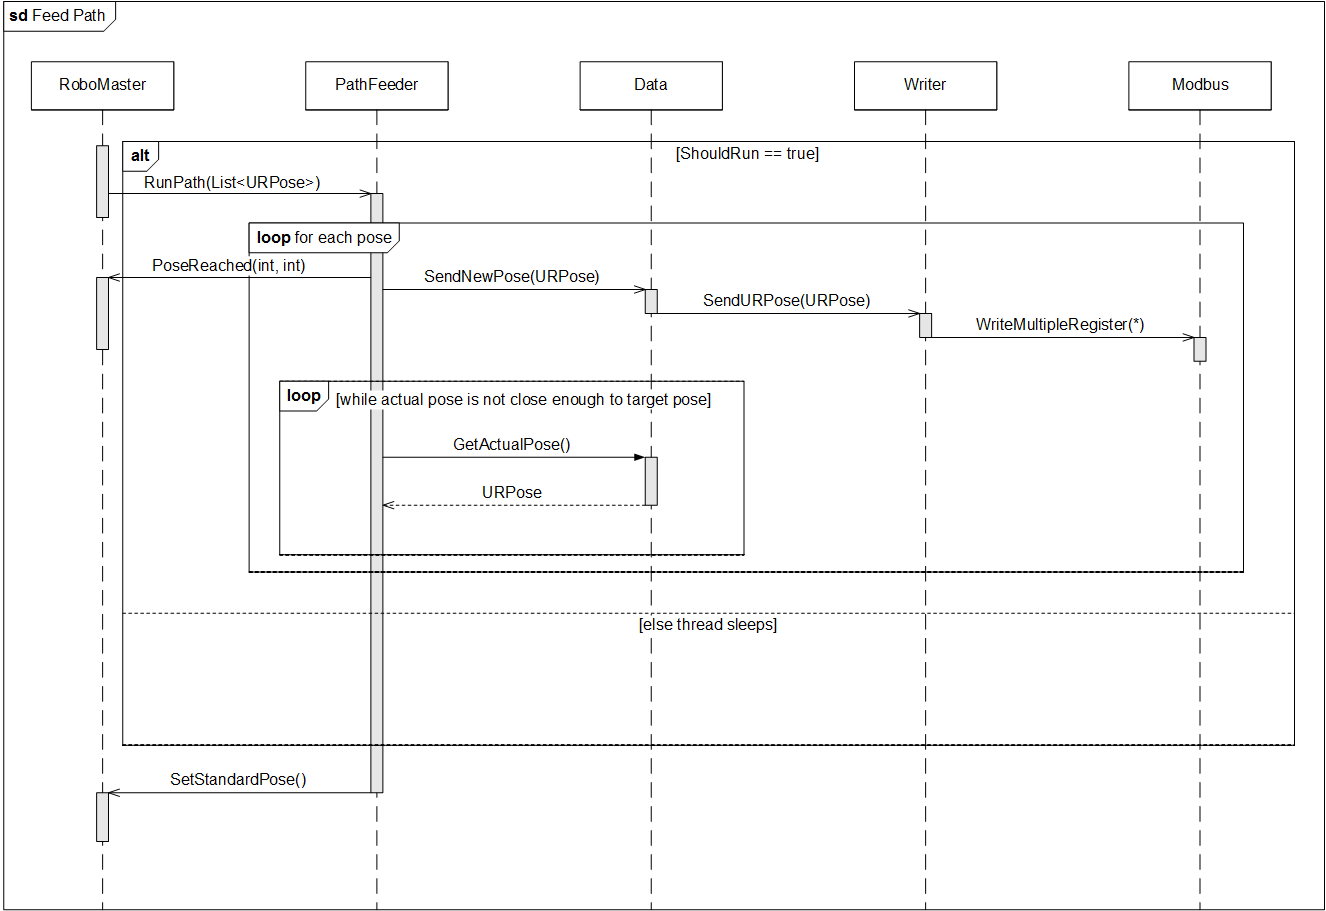
\includegraphics[width=1\textwidth]{figurer/d/Design/Sequence/sd_feedpath}
    \caption{Sekvensdiagram for Feed Path}
    \label{sd_feedpath}
\end{figure}

\subsection{Pathcreation}
Ved tryk på Ultralydsscan-knappen sendes den scannede mesh videre til CalculationMaster. Se sekvensdiagrammet '3D scan' for at se hvordan den scannede mesh opnås.
Først skal meshen konverteres fra 3D Kameras rum til Robot Arms rum, dette sker i CameraToRobotCalibrator, hvor meshen roteres og translateres ift. hvor 3D Kamera befinder sig i virkeligheden.
Efter transformationen skal meshen udjævnes, så de rå og ekstreme normaler i meshen udglattes. Loopet afgør hvor mange gangen meshen skal gennemkøres filteret.
Dernæst sendes den konverterede mesh til PathCreator så der oprettes en liste af de punkter i meshen vi ønsker at Robot Arm skal gennemgå.
Til sidst skal stien der findes i PathCreator konverteres til Robot Arm positurer, da stien i PathCreator kun fortæller position direkte på meshen.
Med denne sti får Robot Arm afdækket overfladen på Patient, hvis den har en Ultralydsscanner monteret.
Stien kan nu videresendes til RoboMaster - se sekvensdiagrammet 'Feed Path' Figur \ref{sd_feedpath}.

\begin{figure}[H]
    \centering
    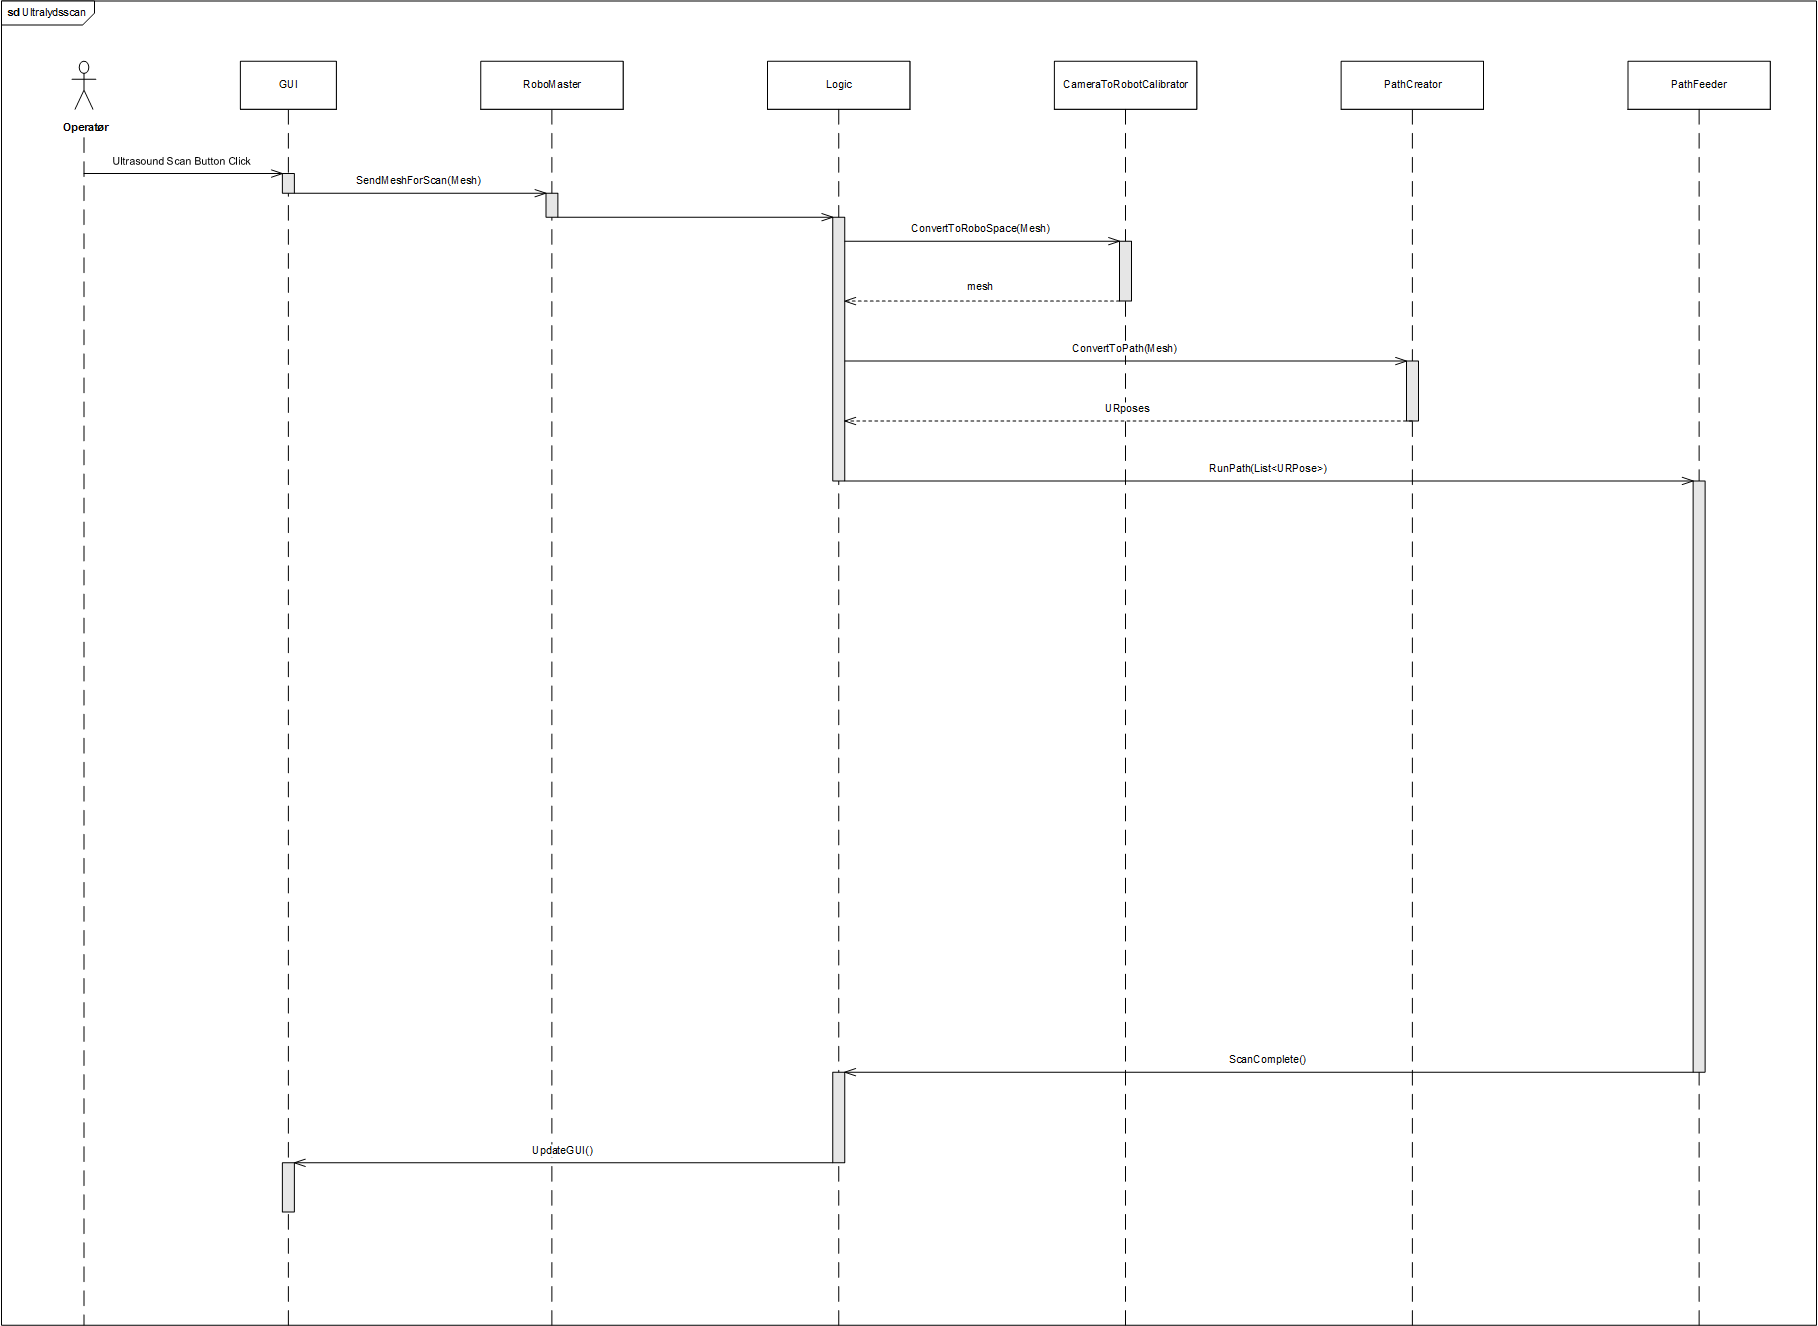
\includegraphics[width=1.4\textwidth, angle =90]{figurer/d/Design/Sequence/sd_ultrascan}
    \caption{Sekvensdiagram for Pathcreation}
    \label{sd_ultrascan}
\end{figure}
\newpage

\section{Detajleret specifikation af klassediagrammer}
Her skal der vises metoderne i hver klasse. 

\section{Tilstandsdiagram}
Dette afsnit beskriver adfærden i systemet ved brug af et tilstandsdiagram. Tilstandsdiagrammet beskriver overgange mellem forskellige tilstande. I UC3: Ultralydsscan brystområde kan Operatør vælge at pause scanningen midlertidig og enten genoptage eller helt stoppe scanning. Figur \ref{stm_Ultra} beskriver Robotarms forskellige tilstande under udførelse af ultralydsscanning. 

\begin{figure}[H]
    \centering
    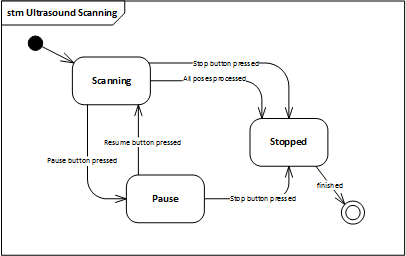
\includegraphics[width=0.7\textwidth]{figurer/d/Design/stm_UC3}
    \caption{Tilstandsdiagram for ultralydsscanning}
    \label{stm_Ultra}
\end{figure}




\chapter{Udviklingsmiljø}\label{Udviklingsvarktojer}

I projektet blev Microsoft Visual Studio 2013 og kodesproget C\# anvendt til at udvikle PC Applikation. 
 
Til debugging er MeshLab og Notepad++ anvendt. 

Google SketchUp version 16.1, er et 3D moduleringsprogam, som i projektet er blevet anvendt til beregninger på 3D modeller detekteret af 3D kamera. 

Til 3D visualisering af Automatisk Ultralydsscanner blev Unity 5.1 anvendt. Hvilket gjorde det nemmere at finde ud af hvad 3D kameras offset var. 

Til matematiske beregninger af Robotarms rotation blev Mathcad 14 anvendt.
\chapter{Implementering}\label{Implementering}
Her beskrives kort hvordan projektets HW-dele og SW-dele er implementeret (”lavet”). HW-delene kan med fordel beskrives med få, udvalgte fotos. Her be-skrives også kort hvordan SW-delene er implementeret (kodet). Den/de an-vendte compilere beskrives kort (programmeringssprog, version etc.). Der ar-gumenteres for valg af programmeringssprog. Der vises kun source code i pro-jektrapporten, når der er tale om ekstremt interessante, små kodeudsnit. Der henvises til projektets bilag, hvor fotos af projektet HW og den samlede source code for projektets SW er anbragt. Beskrivelsen af implementering fylder ty-pisk 1-2 sider.


\chapter{Test}\label{Test}
I dette afsnit beskrives, hvordan systemet er testet for at sikre, at design og implementeringen lever op til systemkrav, defineret i kravspecifikation bilag \ref{Kravspecifikation}. Der er både udført en accepttest (bilag \ref{Accepttest})  for hele systemet Automatisk Ultralydsscanner og unittest (bilag \ref{Udviklingsdokument} af softwaren i PC Applikation. 

\section{Accepttest}
Accepttesten er lavet for at teste funktionelle og ikke-funktionelle krav, som er beskrevet i kravspecifikation. Testen udføres typisk overfor en kunde, men i bachelorprojektet er accepttesten udførst med vejleder, Michael Alrøe. En godkendt test betyder fejlfri gennemførsel, mens ikke godkendt betyder, at teststeppet ikke kan gennemføres og godkendes. Fejl og årsager er nærmere beskrevet i et andet bilag (HUSK REFERENCE, HVIS DER LAVES ET DOKUMENT!). 

Til accepttesten er der benyttet et testobjekt, udformet som et bryst, som erstatning for patient. For at teste Automatisk Ultralydsscanner bevægelsesmønster, er det valgt at påmontere en ”marker!!!!”, som markerer probens bane over testobjektet. 

\subsection{Funktionelle krav} 
Test af funktionelle krav inkluderer syv forskellige test, da både hovedforløb, udtagelser, og udvidelser i de fire use cases skal testes. Nedenstående tabel viser de forskellige tests, der er udført. 

\begin{table}[htb]
\centering
\begin{tabular}{ | l | p{0.80\textwidth} | }
\hline
\textbf{Testens navn} \\\hline
UC1: Hovedscenarie\\\hline 
UC2: Hovedscenarie \\\hline 
UC2: Undtagelse: Juster 3D billedets skæring \\\hline 
UC3: Hovedscenarie \\\hline 
UC3: Udvidelse: Operatør pauser scanning \\\hline 
UC3: Undtagelse: Operatør stopper scanning \\\hline 
UC4: Hovedscenarie \\\hline 
\end{tabular}
\caption{Test af funktionelle krav} 
\end{table}

Se bilag \ref{Accepttest} Accepttest for det fulde testsetup og resultater af hver test. 

\subsection{Ikke-funktionelle krav} 
De ikke-funktionelle krav er MoSCoW-metoden benyttet til at prioritere kravenes vigtighed. Det er valgt kun at teste ’must’-kravene, som kan ses i nedenstående tabel. 

\begin{table}[htb]
\centering
\begin{tabular}{ | c | p{0.80\textwidth} | }
\hline
\textbf{Type} & \textbf{Navn} \\\hline
Usability & U1. PC Applikation skal have en GUI \\\hline 
Performance & P1. Scanningen med 3D kamera og ultralydsscanning skal max tage 10
minutter til sammen \\\hline 
Performance & P2. Startoptid på PC Applikation skal være max 30 sekunder \\\hline
Performance & P3. 3D kamera skal max bruge 1 minut om at tage 3D billedet \\\hline 
Performance & P4. PC Applikation skal max bruge 1 minut på at færdiggøre brystområdets
positurer til Robotarm \\\hline 
Performance & P5. Ultralydsproben skal bevæges over brystet fra højre mod venstre i en
sinus-lignende kurve \\\hline 
\end{tabular}
\caption{Test af funktionelle krav}
\end{table}

Se bilag Accepttest for det fulde testsetup og resultater for hver test. 

\subsection{Unittest af PC Applikation}
Der er undervejs i udviklingen af PC Applikationen udført unittest af softwarens forskellige dele. 
Testene er lavet i et separat projekt, hvad er code coverage procenten på mm. 

Mere skal skrives herunder. 

Se bilag \ref{Udviklingsdokument} Udviklingsdokument, afsnit 'Test' for en uddybning af de forskellige unittests. 

\subsection{Integrationstest}
\chapter{Resultater}\label{kapitel_Resultater}
I dette afsnit er projektets resultat fra accepttesten beskrevet. De opnåede resultater er dokumenteret i accepttest-dokumentet og der henvises derfor til Bilag \ref{Accepttest} Accepttest, for detaljeret beskrivelse af accepttesten. 

\section{Automatisk Ultralydsscanner}
I accepttesten blev de funktionelle og ikke-funktionelle krav for Automatisk Ultralydsscanner testet. Resultatet af accepttesten var at alle tests blev godkendt, på nær UC3: Hovedscenarie. Se Tabel \ref{funk} og \ref{ikke}. 

\subsection{Funktionelle krav}
De funktionelle krav for Automatisk Ultralydsscanner blev godkendt ved test af use cases. 
\begin{table}[htb]
\centering
\begin{tabular}{ | l | p{0.20\textwidth} | }
\hline
\textbf{Testens navn} & \textbf{Godkendt} \\\hline
UC1: Hovedscenarie & \checkmark \\\hline 
UC2: Hovedscenarie & \checkmark \\\hline 
UC2: Undtagelse: Juster 3D billedets skæring & \checkmark \\\hline 
UC3: Hovedscenarie & - \\\hline 
UC3: Udvidelse: Operatør pauser scanning & \checkmark \\\hline 
UC3: Undtagelse: Operatør stopper scanning & \checkmark \\\hline 
UC4: Hovedscenarie & \checkmark \\\hline 
\end{tabular}
\caption{Funktionelle krav}\label{funk} 
\end{table}

Automatisk Ultralydsscanner blev udviklet så det er muligt for Operatør at interagere med PC Applikation, udføre en 3D scanning, og instruere Robotarm om at udføre en ultralydsscanning. 3D billedet kan afgrænses og ultralydsscanningen kan pauses og stoppes. 

Det var ikke muligt for Robotarm at køre i det specifikke bevægelsesmønster beskrevet i bilag \ref{Kravspecifikation} Kravspecifikation og dette var grunden til at UC3: Hovedsenarie fejlede i punkt 2.1 - Testperson observerer, om Robotarm roterer omkring Testobjekt i et specifikt bevægelsesmønster. 
\newpage

\subsection{Ikke-funktionelle krav}
De ikke-funktionelle krav for Automatisk Ultralydsscanner blev godkendt ved test af must-krav. 
 
\begin{table}[htb]
\centering
\begin{tabular}{| l | p{0.65\textwidth}| l |}
\hline
\textbf{Type} & \textbf{Navn} & \textbf{Godkendt}\\\hline
Usability & U1. PC Applikation skal have en GUI & \checkmark \\\hline 
Performance & P1. Scanningen med 3D kamera og ultralydsscanning skal max tage 10
minutter til sammen & \checkmark \\\hline 
Performance & P2. Startoptid på PC Applikation skal være max 30 sekunder & \checkmark \\\hline
Performance & P3. 3D kamera skal max bruge 1 minut om at tage 3D billedet & \checkmark \\\hline 
Performance & P4. PC Applikation skal max bruge 1 minut på at færdiggøre brystområdets
positurer til Robotarm & \checkmark \\\hline 
\end{tabular}
\caption{Ikke-funktionelle krav}\label{ikke}
\end{table}

Det vil sige at PC Applikation blev udviklet med en GUI, det var muligt at udføre en 3D scanning og ultralydsscanning på 3 minutter. Starttiden på PC Applikation var under 30 sekunder, det tog under et minut at tage et 3D billede og PC Applikation brugte under 1 minut på at færdiggøre positurer til ultralydsscanning af brystområdet.  

For at detaljerede resultater af accepttest se bilag \ref{Accepttest} Accepttest. 
\chapter{Diskussion}\label{kapitel_Diskussion}
Med Automatisk Ultralydsscanner er det opnået at lave et system, der kan lave et 3D billede af et testobjekt og derefter få Robotarm til at rotere omkring dette. Alle funktionelle og ikke-funktionelle krav på nær hovedscenariet i UC3: Ultralydsscan brystområdet blev godkendt i accepttesten. 

Det var ikke muligt for Robotarm at udføre bevægelser i det specifikke bevægelsesmønster, beskrevet i Bilag \ref{Kravspecifikation} Kravspecifikation, hvilket gjorde, at UC3: Hovedscenarie fejlede accepttesten. Det betyder ikke, at Robotarm ikke kan bevæge sig over det område som 3D kamera har detekteret, men at det ikke har været muligt at implementere det specifikke bevægelsesmønster nævnt på side \pageref{Probensbevagelse}. Robotarmens bane over brystet er begrænset af 3D kameras detektering af overfladen, hvor der kan opstå ujævnheder. Det er i PC applikationen forsøgt at lave en gennemsnitlig overflade med en udglatningsfunktion for at undgå ujævnheder, da 3D kameraet er upræcist. Dette resulterer i, at de punkter Robotarm benytter som pejlemærker også er upræcise. Det vil være nødvendigt at anvende et mere præcist kamera, bedre udjævningsalgoritmer samt en mere nøge bestemmelse af stien Robotarm skal dække. Derudover vil det være en stor fordel at montere kameraet på Robotarms yderste led, da dette vil give mulighed for at se testobjektet fra blinde vinkler.

For at bestemme rotationen af Robotarms TCP, er der lavet pitch, yaw og roll beregninger, som er implementeret i PC Applikation. En bivirkning af beregningen er at Robotarms yderste led roterer. Dette er uønsket af to grunde: En radiolog vil aldrig rotere en ultralydsprobe på denne måde, og det betyder at Robotarm kan over- eller underrotere dette led. Dette resulterer i at Robotarm stopper op i løbet af en ultralydsscanning. Det er endnu ikke lykkedes at finde en løsning på dette problem.

Det var nødvendigt at give Operatør mulighed for at kunne se og godkende billedet fra 3D kameraet, da der er tilfælde, hvor 3D scanningen ikke bliver udført som forventet. Derfor blev det valgt at vise dybdebilledet og 3D scanningen i selve GUI'en. Med disse to billeder vil Operatør nemmere kunne justere på værdier der afgrænser området der skal scannes, for ikke at ultralydsscanne noget der ikke er brystvæv.

I projektet er performancetiderne til systemet blevet prioriteret højt, da det potentielt vil kunne forbedre mulighederne for implementering af systemet i sundhedsvæsenet, hvor tid er en vigtig resurse. Til accepttesten tog det systemet omkring 3 minutter for at afvikle først 3D scanning og derefter rotere Robotarm rundt på området, hvor det i kravspecifikationen bilag \ref{Kravspecifikation} er et krav, at det må tage 10 minutter til sammen. En 3D scanning er sat til at må tage 10 sekunder, men til accepttesten tog det omkring 2 sekunder at vise 3D billedet på GUI. PC Applikation brugte under 1 sekund i stedet for de 10 sekunder, for at færdiggøre brystområdets positurer til Robotarm. Performancetiderne lå generelt et godt stykke under kravene defineret ud fra interviews med radiolog Lars Bolvig og afdelingsradiograf Tine Bisgaard, men for at kunne tages i brug, er der flere faktorer. Men performance-tiden er meget afhængig af de beslutninger der tages for hvor høj kvaliteten af ultralydsscanningen skal være. En højere opløsning på 3D scanningen samt flere gennemgange af udjævningsalgoritmen vil øge den tid PC Applikationen bruger på at finde positurer betydeligt.  

Der er mangel på radiologer i Danmark, såvel som resten af verden \ref{Lagemangel}, hvorfor man skal tænke andre metoder og arbejdsgange. På længere sigt kan man forestille sig, at radiografer overtager nogle af opgaverne fra radiologerne, heriblandt bl.a. ultralydsscanninger. Ved f.eks. at lade radiografer lave selve scanningerne, vil patienter først få besked efter radiologen har tilset scanningerne. Den procedure er også brugt til mammografi med røntgen. Det kan diskuteres, om en udvidelse af screeningsprogrammet vil være en god ting: Udvidelsen vil give mulighed for at finde flere kræfttilfælde - men der er risiko for overbehandling og øgede udgifter til sundhedsvæsenet. Man kunne i stedet forestille sig, at en del af røntgenscanningerne kunne erstattes af ultralydsscanninger, da 1 ud af 100.000 !!HUSK REF patienter udvikler kræft røntgenstråling, mens der ikke er nogen kendte bivirkninger ved ultralydsscanninger af brystet. Røntgenundersøgelser er billigere !!HUSK REF end ultralydsundersøgelser, bl.a. fordi at en radiolog laver scanningerne. 

Den medicinske godkendelse burde have været implementeret i kravspecifikationens funktionelle krav til Automatisk Ultralydsscanner, for at overholde lovgivning til CE-mærkning. Det blev besluttet at prioritere udviklingen af Automatisk Ultralydsscanner højere end den medicinske godkendelse, da bachelorprojektet skulle undersøge selve muligheden for at udvikle et system til automatiseret ultralydsscanning af mamma mhp. screening for brystkræft. Den medicinske godkendelse vil derfor kunne have været en forhindring i denne udviklingsproces, og andre krav ville ikke være blevet implementeret. 

Hvis et system til automatisk ultralydsscanning af brystet skal medicinsk godkendes er det vigtigt først at tjekke, om hver komponent er godkendt til medicinsk brug, for at kunne bruge det i kombination med hele systemet. At få en medicinsk godkendelse kan tage mange år, og pt. er UR10 ikke godkendt til medicinsk brug. Derfor kan det være bedre at udvikle systemet til automatisk ultralydsscanning på en robot, der allerede er godkendt til medicinsk brug. 
\chapter{Fremtidig udvikling}\label{kapitel_Fremtidig udvikling}

Næste skridt i udviklingen af Automatisk Ultralydsscaner vil være software til tryk-korrigering.
Dette vil give mulighed for at variere det tryk som Robotarm leverer på brystet. Trykvariation er nødvendigt for at udføre en ultralydsscanning, da ultralydssproben kun kan lave en brugbar ultralydsscanning ved et bestemt tryk. 
I nuværende version vil Robotarm stoppe, hvis den trykker for hårdt, altså hvis trykket kommer over den tærskelværdi der er givet. Samtidig vil Robotarm heller ikke tage højde for hvis den slet ikke leverer noget tryk.
Det kan være at tryk-værdierne fra Robotarm ikke er brugbare nok og man derfor ud over software ville være tvunget til at bruge en yderligere tryksensor.

For at Automatisk Ultralydscanner skal kunne foretage en fuld scanning, vil det også være nødvendigt med flere vinkler fra 3D kamera. Automatisk Ultralydsscanner er begrænset til at kunne scanne det område af brystet, som 3D kameraet kan detektere. I nuværende version er 3D kamera monteret fast til loftet. Her vil det være ideelt at Robotarm har 3D kamera monteret, så flere 3D billeder fra samme 3D kamera kan kombineres.

Automatisk Ultralydsscanner blev udviklet med det formål at lave ultralydsscanning til en simpel procedure, hvor radiologen i mindre grad var en del af systemet. Derfor kunne der være et scenario i fremtiden, hvor systemet selv kan finde knuder gennem billedgenkendelse. Derved vil radiologen kunne varetage vigtigere opgaver, og patienten kan få svar allerede inde ved konsultationen i stedet for at vente.

Hvis Automatisk Ultralydsscanner skal anvendes på hospitaler, vil det være nødvendigt at integrere et login til operatør, samt lave identifikation i form af CPR-nummer i PC Applikationen. Systemet skal derfor også kunne gemme målinger sikkert i en database. 

I fremtiden kunne det også være en stor fordel, hvis man kunne anvende Automatisk Ultralydsscanner til andre simple procedurer. For eksempel flowmåling i arme og ben, hvilket formentligt ikke vil kræve andet udstyr end det, der er anvendt i bachelorprojektet. En Automatisk Ultralydsscanner kan i sin nuværende form ikke anvendes til scanninger in vivo.

Det vil også være nødvendigt at udføre kravene til medicinsk godkendelse, for at få Automatisk Ultralydsscanner CE-mærket. Dette vil blandt andet indebære udvikling af kvalitetssikringsystem, risikovurdering, overholdelse af væsentlige krav fra MDD. Derudover skal der udføres test for Elektromagnetisk stråling, bio-kompatibilitetstestes og klinisk test på Automatisk Ultralydsscanner, samt klinisk evaluering. 

\chapter{Konklusion}\label{kapitel_Konklusion}
Automatiseret Ultralydsscanner er i stand til at detektere et brystområde med 3D kameraet og derefter bevæge robotarmen rundt på området, men systemet er i sin nuværende form ikke i stand til at lave professionelle scanninger for brystkræft. En radiolog, der scanner for brystkræft vil føre ultralydsproben i et specifikt bevægelsesmønster over hele brystet og i armhulen, hvilket Automatisk Ultralydsscanner ikke er i stand til. Automatisk Ultralydsscanner er begrænset til kun at kunne scanne et detekteret område, som er scannet af 3D Kamera monteret i loftet, hvorfor hele brystets form og armhule placering ikke bliver detekteret. Automatisk Ultralydsscanner kan ikke registrere, hvor hårdt der trykkes på patienten, hvilket en automatiseret ultralydsscanner mhp. på screening for brystkræft bør have ift. patientsikkerhed. 

En automatiseret ultralydsscanning kan gavne økonomisk, hvis der allokeres opgaver fra radiologer til radiografer, da der er stor forskel på timelønnen. Den automatiserede ultralydsscanning af mamma kan foretages af radiografer, hvorefter radiologen vil sidde og vurdere scanningerne, ligesom proceduren er ved mammografiscreeninger. Denne model vil kunne spare transporttid for radiologen, og prisen pr. ultralydsscanning vil dermed blive lavere.  

Inden Automatisk Ultralydsscanner kan CE-mærkes, skal producenten overholde væsentlige krav fra DMD. Der skal udarbejdes teknisk dokumentation for produktet, bestående af en risikoanalyse og klinisk evaluering. Der vil skulle laves et kvalitetssikringssystem og have post market surveillance system. Derudover er det vigtigt at vælge et bemyndiget organ, som godkender, at dokumentationen lever op til gældende lovgivning. Disse krav er ikke blevet implementeret i Automatisk Ultralydsscanner, da kendskabet til MDD først kom efter udviklingsprocessen var startet.

På Aarhus Universitetshospital, Tage-Hansens Gade, var man positive overfor en automatiserede ultralydssanning, da det kan give økonomisk mening og afhjælpe problemet med manglen på radiologer. Der vil være risiko for, at radiologen vil bruge mere tid på at analysere og vurdere billederne. 
De potentielle patienter fra spørgeskemaundersøgelsen var generelt positive overfor et system, og de fremhævede vigtigheden ved robottens følsomhed overfor tryk. Der blev det formodet , at en automatiseret ultralydsscanning vil kunne give økonomisk mening med kortere ventetider, spare tid og dermed frigørelse af ressourcer i form af personale til andre opgaver. 


\backmatter
\chapter{Bilag}\label{Bilag}

\ref{Satningsliste} Sætningsliste \\
\ref{UR10spec} UR10 Specifikation \\
%\refl{UserManualUR10}


\bibliographystyle{plain}
\bibliography{bibliografi/PRJ3}    % Sætter bibliografien bagerst i dokumentet. Bruger bib-filen PRJ3.

\end{document}
